% Options for packages loaded elsewhere
\PassOptionsToPackage{unicode}{hyperref}
\PassOptionsToPackage{hyphens}{url}
\PassOptionsToPackage{dvipsnames,svgnames,x11names}{xcolor}
%
\documentclass[
  letterpaper,
  DIV=11,
  numbers=noendperiod]{scrartcl}

\usepackage{amsmath,amssymb}
\usepackage{iftex}
\ifPDFTeX
  \usepackage[T1]{fontenc}
  \usepackage[utf8]{inputenc}
  \usepackage{textcomp} % provide euro and other symbols
\else % if luatex or xetex
  \usepackage{unicode-math}
  \defaultfontfeatures{Scale=MatchLowercase}
  \defaultfontfeatures[\rmfamily]{Ligatures=TeX,Scale=1}
\fi
\usepackage{lmodern}
\ifPDFTeX\else  
    % xetex/luatex font selection
\fi
% Use upquote if available, for straight quotes in verbatim environments
\IfFileExists{upquote.sty}{\usepackage{upquote}}{}
\IfFileExists{microtype.sty}{% use microtype if available
  \usepackage[]{microtype}
  \UseMicrotypeSet[protrusion]{basicmath} % disable protrusion for tt fonts
}{}
\makeatletter
\@ifundefined{KOMAClassName}{% if non-KOMA class
  \IfFileExists{parskip.sty}{%
    \usepackage{parskip}
  }{% else
    \setlength{\parindent}{0pt}
    \setlength{\parskip}{6pt plus 2pt minus 1pt}}
}{% if KOMA class
  \KOMAoptions{parskip=half}}
\makeatother
\usepackage{xcolor}
\setlength{\emergencystretch}{3em} % prevent overfull lines
\setcounter{secnumdepth}{5}
% Make \paragraph and \subparagraph free-standing
\ifx\paragraph\undefined\else
  \let\oldparagraph\paragraph
  \renewcommand{\paragraph}[1]{\oldparagraph{#1}\mbox{}}
\fi
\ifx\subparagraph\undefined\else
  \let\oldsubparagraph\subparagraph
  \renewcommand{\subparagraph}[1]{\oldsubparagraph{#1}\mbox{}}
\fi

\usepackage{color}
\usepackage{fancyvrb}
\newcommand{\VerbBar}{|}
\newcommand{\VERB}{\Verb[commandchars=\\\{\}]}
\DefineVerbatimEnvironment{Highlighting}{Verbatim}{commandchars=\\\{\}}
% Add ',fontsize=\small' for more characters per line
\usepackage{framed}
\definecolor{shadecolor}{RGB}{241,243,245}
\newenvironment{Shaded}{\begin{snugshade}}{\end{snugshade}}
\newcommand{\AlertTok}[1]{\textcolor[rgb]{0.68,0.00,0.00}{#1}}
\newcommand{\AnnotationTok}[1]{\textcolor[rgb]{0.37,0.37,0.37}{#1}}
\newcommand{\AttributeTok}[1]{\textcolor[rgb]{0.40,0.45,0.13}{#1}}
\newcommand{\BaseNTok}[1]{\textcolor[rgb]{0.68,0.00,0.00}{#1}}
\newcommand{\BuiltInTok}[1]{\textcolor[rgb]{0.00,0.23,0.31}{#1}}
\newcommand{\CharTok}[1]{\textcolor[rgb]{0.13,0.47,0.30}{#1}}
\newcommand{\CommentTok}[1]{\textcolor[rgb]{0.37,0.37,0.37}{#1}}
\newcommand{\CommentVarTok}[1]{\textcolor[rgb]{0.37,0.37,0.37}{\textit{#1}}}
\newcommand{\ConstantTok}[1]{\textcolor[rgb]{0.56,0.35,0.01}{#1}}
\newcommand{\ControlFlowTok}[1]{\textcolor[rgb]{0.00,0.23,0.31}{#1}}
\newcommand{\DataTypeTok}[1]{\textcolor[rgb]{0.68,0.00,0.00}{#1}}
\newcommand{\DecValTok}[1]{\textcolor[rgb]{0.68,0.00,0.00}{#1}}
\newcommand{\DocumentationTok}[1]{\textcolor[rgb]{0.37,0.37,0.37}{\textit{#1}}}
\newcommand{\ErrorTok}[1]{\textcolor[rgb]{0.68,0.00,0.00}{#1}}
\newcommand{\ExtensionTok}[1]{\textcolor[rgb]{0.00,0.23,0.31}{#1}}
\newcommand{\FloatTok}[1]{\textcolor[rgb]{0.68,0.00,0.00}{#1}}
\newcommand{\FunctionTok}[1]{\textcolor[rgb]{0.28,0.35,0.67}{#1}}
\newcommand{\ImportTok}[1]{\textcolor[rgb]{0.00,0.46,0.62}{#1}}
\newcommand{\InformationTok}[1]{\textcolor[rgb]{0.37,0.37,0.37}{#1}}
\newcommand{\KeywordTok}[1]{\textcolor[rgb]{0.00,0.23,0.31}{#1}}
\newcommand{\NormalTok}[1]{\textcolor[rgb]{0.00,0.23,0.31}{#1}}
\newcommand{\OperatorTok}[1]{\textcolor[rgb]{0.37,0.37,0.37}{#1}}
\newcommand{\OtherTok}[1]{\textcolor[rgb]{0.00,0.23,0.31}{#1}}
\newcommand{\PreprocessorTok}[1]{\textcolor[rgb]{0.68,0.00,0.00}{#1}}
\newcommand{\RegionMarkerTok}[1]{\textcolor[rgb]{0.00,0.23,0.31}{#1}}
\newcommand{\SpecialCharTok}[1]{\textcolor[rgb]{0.37,0.37,0.37}{#1}}
\newcommand{\SpecialStringTok}[1]{\textcolor[rgb]{0.13,0.47,0.30}{#1}}
\newcommand{\StringTok}[1]{\textcolor[rgb]{0.13,0.47,0.30}{#1}}
\newcommand{\VariableTok}[1]{\textcolor[rgb]{0.07,0.07,0.07}{#1}}
\newcommand{\VerbatimStringTok}[1]{\textcolor[rgb]{0.13,0.47,0.30}{#1}}
\newcommand{\WarningTok}[1]{\textcolor[rgb]{0.37,0.37,0.37}{\textit{#1}}}

\providecommand{\tightlist}{%
  \setlength{\itemsep}{0pt}\setlength{\parskip}{0pt}}\usepackage{longtable,booktabs,array}
\usepackage{calc} % for calculating minipage widths
% Correct order of tables after \paragraph or \subparagraph
\usepackage{etoolbox}
\makeatletter
\patchcmd\longtable{\par}{\if@noskipsec\mbox{}\fi\par}{}{}
\makeatother
% Allow footnotes in longtable head/foot
\IfFileExists{footnotehyper.sty}{\usepackage{footnotehyper}}{\usepackage{footnote}}
\makesavenoteenv{longtable}
\usepackage{graphicx}
\makeatletter
\def\maxwidth{\ifdim\Gin@nat@width>\linewidth\linewidth\else\Gin@nat@width\fi}
\def\maxheight{\ifdim\Gin@nat@height>\textheight\textheight\else\Gin@nat@height\fi}
\makeatother
% Scale images if necessary, so that they will not overflow the page
% margins by default, and it is still possible to overwrite the defaults
% using explicit options in \includegraphics[width, height, ...]{}
\setkeys{Gin}{width=\maxwidth,height=\maxheight,keepaspectratio}
% Set default figure placement to htbp
\makeatletter
\def\fps@figure{htbp}
\makeatother

\KOMAoption{captions}{tableheading}
\makeatletter
\@ifpackageloaded{tcolorbox}{}{\usepackage[skins,breakable]{tcolorbox}}
\@ifpackageloaded{fontawesome5}{}{\usepackage{fontawesome5}}
\definecolor{quarto-callout-color}{HTML}{909090}
\definecolor{quarto-callout-note-color}{HTML}{0758E5}
\definecolor{quarto-callout-important-color}{HTML}{CC1914}
\definecolor{quarto-callout-warning-color}{HTML}{EB9113}
\definecolor{quarto-callout-tip-color}{HTML}{00A047}
\definecolor{quarto-callout-caution-color}{HTML}{FC5300}
\definecolor{quarto-callout-color-frame}{HTML}{acacac}
\definecolor{quarto-callout-note-color-frame}{HTML}{4582ec}
\definecolor{quarto-callout-important-color-frame}{HTML}{d9534f}
\definecolor{quarto-callout-warning-color-frame}{HTML}{f0ad4e}
\definecolor{quarto-callout-tip-color-frame}{HTML}{02b875}
\definecolor{quarto-callout-caution-color-frame}{HTML}{fd7e14}
\makeatother
\makeatletter
\makeatother
\makeatletter
\makeatother
\makeatletter
\@ifpackageloaded{caption}{}{\usepackage{caption}}
\AtBeginDocument{%
\ifdefined\contentsname
  \renewcommand*\contentsname{Table of contents}
\else
  \newcommand\contentsname{Table of contents}
\fi
\ifdefined\listfigurename
  \renewcommand*\listfigurename{List of Figures}
\else
  \newcommand\listfigurename{List of Figures}
\fi
\ifdefined\listtablename
  \renewcommand*\listtablename{List of Tables}
\else
  \newcommand\listtablename{List of Tables}
\fi
\ifdefined\figurename
  \renewcommand*\figurename{Figure}
\else
  \newcommand\figurename{Figure}
\fi
\ifdefined\tablename
  \renewcommand*\tablename{Table}
\else
  \newcommand\tablename{Table}
\fi
}
\@ifpackageloaded{float}{}{\usepackage{float}}
\floatstyle{ruled}
\@ifundefined{c@chapter}{\newfloat{codelisting}{h}{lop}}{\newfloat{codelisting}{h}{lop}[chapter]}
\floatname{codelisting}{Listing}
\newcommand*\listoflistings{\listof{codelisting}{List of Listings}}
\makeatother
\makeatletter
\@ifpackageloaded{caption}{}{\usepackage{caption}}
\@ifpackageloaded{subcaption}{}{\usepackage{subcaption}}
\makeatother
\makeatletter
\@ifpackageloaded{tcolorbox}{}{\usepackage[skins,breakable]{tcolorbox}}
\makeatother
\makeatletter
\@ifundefined{shadecolor}{\definecolor{shadecolor}{rgb}{.97, .97, .97}}
\makeatother
\makeatletter
\makeatother
\makeatletter
\makeatother
\ifLuaTeX
  \usepackage{selnolig}  % disable illegal ligatures
\fi
\IfFileExists{bookmark.sty}{\usepackage{bookmark}}{\usepackage{hyperref}}
\IfFileExists{xurl.sty}{\usepackage{xurl}}{} % add URL line breaks if available
\urlstyle{same} % disable monospaced font for URLs
\hypersetup{
  pdftitle={Análisis IPs},
  pdfauthor={Garcia Justo},
  colorlinks=true,
  linkcolor={blue},
  filecolor={Maroon},
  citecolor={Blue},
  urlcolor={Blue},
  pdfcreator={LaTeX via pandoc}}

\title{Análisis IPs}
\author{Garcia Justo}
\date{}

\begin{document}
\maketitle
\ifdefined\Shaded\renewenvironment{Shaded}{\begin{tcolorbox}[interior hidden, enhanced, frame hidden, borderline west={3pt}{0pt}{shadecolor}, sharp corners, boxrule=0pt, breakable]}{\end{tcolorbox}}\fi

\hypertarget{anuxe1lisis-de-ips-reportadas-como-atacantes-por-ssh}{%
\subsection{Análisis de IPs reportadas como atacantes por
SSH}\label{anuxe1lisis-de-ips-reportadas-como-atacantes-por-ssh}}

Los ataques por SSH (Secure Shell) son intentos maliciosos de
comprometer un sistema a través del protocolo SSH.

\begin{figure}

{\centering 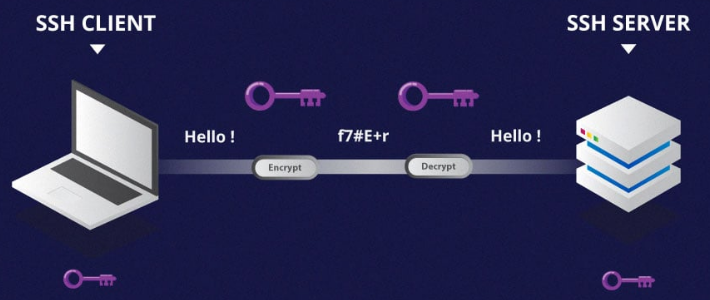
\includegraphics{imagenes/ssh.png}

}

\caption{Protocolo SSH}

\end{figure}

SSH es muy utilizado porque permite establecer una conexión segura y
cifrada entre un cliente y un servidor. Pero, establecida la conexión,
puede ser también aprovechado por los atacantes.

Dado que es información proporcionada, no se sabe la naturaleza del
ataque, pero entre los más comunes estan los de fuerza bruta.

\hypertarget{extracciuxf3n-de-ips}{%
\subsubsection{Extracción de IPs}\label{extracciuxf3n-de-ips}}

Para la realización de este análisis la cátedra proporcionó una lista de
IPs que fueron reportadas por conexiones SSH y ataques DDoS. En este
caso extraeré las IPs de SSH.

\begin{Shaded}
\begin{Highlighting}[]
\NormalTok{patron }\OperatorTok{=} \StringTok{"[0{-}9]\{1,3\}\textbackslash{}.[0{-}9]\{1,3\}\textbackslash{}.[0{-}9]\{1,3\}\textbackslash{}.[0{-}9]\{1,3\}"}
\OperatorTok{!}\NormalTok{grep }\OperatorTok{{-}}\NormalTok{Eo }\StringTok{"$patron"}\NormalTok{ data}\OperatorTok{/}\NormalTok{SSH.txt }\OperatorTok{\textgreater{}}\NormalTok{ data}\OperatorTok{/}\NormalTok{IPsSSH.txt}
\end{Highlighting}
\end{Shaded}

\begin{Shaded}
\begin{Highlighting}[]
\ControlFlowTok{with} \BuiltInTok{open}\NormalTok{(}\StringTok{"data/IPsSSH.txt"}\NormalTok{) }\ImportTok{as}\NormalTok{ ips:}
\NormalTok{    ipSSH }\OperatorTok{=}\NormalTok{ ips.read()}
    
\NormalTok{ipSSH }\OperatorTok{=}\NormalTok{ ipSSH.replace(}\StringTok{"}\CharTok{\textbackslash{}n}\StringTok{"}\NormalTok{, }\StringTok{" "}\NormalTok{).split()}
\NormalTok{ipSSH}
\end{Highlighting}
\end{Shaded}

\begin{verbatim}
['54.144.244.57',
 '188.166.216.223',
 '220.94.228.162',
 '218.92.0.99',
 '116.193.159.2',
 '109.117.92.13',
 '167.99.112.43',
 '89.248.163.219',
 '143.198.204.177',
 '61.177.173.45',
 '8.222.204.225',
 '220.135.119.188']
\end{verbatim}

\hypertarget{importamos-la-implementaciuxf3n-de-las-peticiones-a-la-api}{%
\subsubsection{Importamos la implementación de las peticiones a la
API}\label{importamos-la-implementaciuxf3n-de-las-peticiones-a-la-api}}

\begin{Shaded}
\begin{Highlighting}[]
\OperatorTok{!}\NormalTok{cp ..}\OperatorTok{/}\NormalTok{app}\OperatorTok{/}\NormalTok{modulos}\OperatorTok{/}\NormalTok{abuseIPDB.py modulos}\OperatorTok{/}\NormalTok{abuseIPDB.py}
\end{Highlighting}
\end{Shaded}

\begin{Shaded}
\begin{Highlighting}[]
\CommentTok{\#Importo los modulos necesarios}
\ImportTok{from}\NormalTok{ modulos.abuseIPDB }\ImportTok{import}\NormalTok{ AbuseIPDB}
\ImportTok{import}\NormalTok{ pandas }\ImportTok{as}\NormalTok{ pd}
\end{Highlighting}
\end{Shaded}

\begin{Shaded}
\begin{Highlighting}[]
\CommentTok{\#Construyo el objeto}
\NormalTok{apiAbuse }\OperatorTok{=}\NormalTok{ AbuseIPDB()}
\end{Highlighting}
\end{Shaded}

\begin{Shaded}
\begin{Highlighting}[]
\ImportTok{import}\NormalTok{ os}
\end{Highlighting}
\end{Shaded}

\begin{Shaded}
\begin{Highlighting}[]
\CommentTok{\#Declaro las keys de la info que devuelve mi implementación de requests}
\NormalTok{keys }\OperatorTok{=}\NormalTok{ [}\StringTok{\textquotesingle{}esPublica\textquotesingle{}}\NormalTok{, }\StringTok{\textquotesingle{}estaEnWhitelist\textquotesingle{}}\NormalTok{, }\StringTok{\textquotesingle{}scoreAbuso\textquotesingle{}}\NormalTok{, }\StringTok{\textquotesingle{}pais\textquotesingle{}}\NormalTok{, }\StringTok{\textquotesingle{}codigoPais\textquotesingle{}}\NormalTok{, }\StringTok{\textquotesingle{}isp\textquotesingle{}}\NormalTok{, }\StringTok{\textquotesingle{}tipoDeUso\textquotesingle{}}\NormalTok{, }\StringTok{\textquotesingle{}ultimoReporte\textquotesingle{}}\NormalTok{]}

\NormalTok{diccDf }\OperatorTok{=}\NormalTok{ \{}\StringTok{\textquotesingle{}ip\textquotesingle{}}\NormalTok{ : []\}}

\ControlFlowTok{if}\NormalTok{ os.path.isfile(}\StringTok{"data/ipSSH.csv"}\NormalTok{):}
    
\NormalTok{    df }\OperatorTok{=}\NormalTok{ pd.read\_csv(}\StringTok{"data/ipSSH.csv"}\NormalTok{)}
    
\ControlFlowTok{else}\NormalTok{:}
    \ControlFlowTok{for}\NormalTok{ ip }\KeywordTok{in}\NormalTok{ ipSSH:}
\NormalTok{        diccDf[}\StringTok{\textquotesingle{}ip\textquotesingle{}}\NormalTok{].append(ip)}
\NormalTok{        info }\OperatorTok{=}\NormalTok{ apiAbuse.getInfo(ip)}
        \ControlFlowTok{for}\NormalTok{ key }\KeywordTok{in}\NormalTok{ keys:}
            \ControlFlowTok{if}\NormalTok{ key }\KeywordTok{in}\NormalTok{ diccDf:}
\NormalTok{                diccDf[key].append(info[key])}
            \ControlFlowTok{else}\NormalTok{:}
\NormalTok{                diccDf[key] }\OperatorTok{=}\NormalTok{ [info[key]]}

\NormalTok{        df }\OperatorTok{=}\NormalTok{ pd.DataFrame(data}\OperatorTok{=}\NormalTok{diccDf)}
\end{Highlighting}
\end{Shaded}

\begin{Shaded}
\begin{Highlighting}[]
\NormalTok{df}
\end{Highlighting}
\end{Shaded}

\begin{longtable}[]{@{}llllllllll@{}}
\toprule\noalign{}
& ip & esPublica & estaEnWhitelist & scoreAbuso & pais & codigoPais &
isp & tipoDeUso & ultimoReporte \\
\midrule\noalign{}
\endhead
\bottomrule\noalign{}
\endlastfoot
0 & 54.144.244.57 & True & False & 58 & NaN & US & Amazon Data Services
NoVa & Data Center/Web Hosting/Transit & 2023-05-24T06:13:13+00:00 \\
1 & 188.166.216.223 & True & False & 100 & NaN & SG & DigitalOcean LLC &
Data Center/Web Hosting/Transit & 2023-05-25T17:08:47+00:00 \\
2 & 220.94.228.162 & True & False & 100 & NaN & KR & KT Corporation &
None & 2023-05-25T22:00:07+00:00 \\
3 & 218.92.0.99 & True & False & 100 & NaN & CN & ChinaNet Jiangsu
Province Network & Data Center/Web Hosting/Transit &
2023-05-25T23:18:56+00:00 \\
4 & 116.193.159.2 & True & False & 100 & NaN & HK & Pacswitch Globe
Telecom Limited & Data Center/Web Hosting/Transit &
2023-05-25T22:00:08+00:00 \\
5 & 109.117.92.13 & True & False & 100 & NaN & IT & Vodafone Italia
S.p.A. & None & 2023-05-25T22:04:00+00:00 \\
6 & 167.99.112.43 & True & False & 100 & NaN & US & DigitalOcean LLC &
Data Center/Web Hosting/Transit & 2023-05-25T22:00:10+00:00 \\
7 & 89.248.163.219 & True & False & 100 & NaN & NL & FiberXpress BV &
Fixed Line ISP & 2023-05-25T23:41:25+00:00 \\
8 & 143.198.204.177 & True & False & 100 & NaN & SG & DigitalOcean LLC &
Data Center/Web Hosting/Transit & 2023-05-25T22:14:42+00:00 \\
9 & 61.177.173.45 & True & False & 100 & NaN & CN & ChinaNet Jiangsu
Province Network & Data Center/Web Hosting/Transit &
2023-05-25T22:05:26+00:00 \\
10 & 8.222.204.225 & True & False & 100 & NaN & SG & Alibaba.com
Singapore E-Commerce Private Limited & Data Center/Web Hosting/Transit &
2023-05-25T22:44:47+00:00 \\
11 & 220.135.119.188 & True & False & 100 & NaN & TW & Chunghwa Telecom
Co. Ltd. & None & 2023-05-25T23:37:31+00:00 \\
\end{longtable}

\begin{Shaded}
\begin{Highlighting}[]
\NormalTok{unameds }\OperatorTok{=}\NormalTok{ [i }\ControlFlowTok{for}\NormalTok{ i }\KeywordTok{in}\NormalTok{ df.columns }\ControlFlowTok{if} \StringTok{\textquotesingle{}Unnamed\textquotesingle{}} \KeywordTok{in}\NormalTok{ i]}
\ControlFlowTok{for}\NormalTok{ i }\KeywordTok{in}\NormalTok{ unameds:}
\NormalTok{    df.drop(i, axis}\OperatorTok{=}\DecValTok{1}\NormalTok{, inplace}\OperatorTok{=}\VariableTok{True}\NormalTok{)}
\NormalTok{df.to\_csv(}\StringTok{"data/ipSSH.csv"}\NormalTok{, index}\OperatorTok{=}\VariableTok{False}\NormalTok{)}
\end{Highlighting}
\end{Shaded}

\hypertarget{uxedndices-de-abuso}{%
\subsubsection{Índices de abuso}\label{uxedndices-de-abuso}}

\begin{Shaded}
\begin{Highlighting}[]
\NormalTok{recuento }\OperatorTok{=}\NormalTok{ df[}\StringTok{"scoreAbuso"}\NormalTok{].value\_counts().to\_dict()}

\NormalTok{pd.DataFrame(data}\OperatorTok{=}\NormalTok{\{}\StringTok{"Score"}\NormalTok{: }\BuiltInTok{list}\NormalTok{(recuento.keys()), }\StringTok{"Reportes"}\NormalTok{: }\BuiltInTok{list}\NormalTok{(recuento.values())\})}
\end{Highlighting}
\end{Shaded}

\hypertarget{tbl-indicesssh}{}
\begin{longtable}[]{@{}lll@{}}
\caption{\label{tbl-indicesssh}Indice de abuso y las veces que se
repite}\tabularnewline
\toprule\noalign{}
& Score & Reportes \\
\midrule\noalign{}
\endfirsthead
\toprule\noalign{}
& Score & Reportes \\
\midrule\noalign{}
\endhead
\bottomrule\noalign{}
\endlastfoot
0 & 100 & 11 \\
1 & 58 & 1 \\
\end{longtable}

Como se puede apreciar en la tabla de arriba, han sido múltiples veces
reportadas por distintos usuarios a lo largo del mundo. Por lo tanto,
tenemos la certeza de que son IPs que han sido utilizadas con fines
malintencionados.

\hypertarget{anuxe1lisis-de-procedencia}{%
\subsubsection{Análisis de
procedencia}\label{anuxe1lisis-de-procedencia}}

\begin{Shaded}
\begin{Highlighting}[]
\ImportTok{import}\NormalTok{ pycountry}
\end{Highlighting}
\end{Shaded}

\begin{Shaded}
\begin{Highlighting}[]
\NormalTok{df[}\StringTok{\textquotesingle{}pais\textquotesingle{}}\NormalTok{] }\OperatorTok{=}\NormalTok{ df[}\StringTok{\textquotesingle{}codigoPais\textquotesingle{}}\NormalTok{].}\BuiltInTok{apply}\NormalTok{(}\KeywordTok{lambda}\NormalTok{ codigo: pycountry.countries.get(alpha\_2}\OperatorTok{=}\NormalTok{codigo).name)}
\NormalTok{dfgdp }\OperatorTok{=}\NormalTok{ df.copy()}
\NormalTok{dfgdp[}\StringTok{\textquotesingle{}codigoPais\textquotesingle{}}\NormalTok{] }\OperatorTok{=}\NormalTok{ df[}\StringTok{\textquotesingle{}pais\textquotesingle{}}\NormalTok{].}\BuiltInTok{apply}\NormalTok{(}\KeywordTok{lambda}\NormalTok{ nombre: pycountry.countries.search\_fuzzy(nombre)[}\DecValTok{0}\NormalTok{].alpha\_3)}
\end{Highlighting}
\end{Shaded}

\begin{Shaded}
\begin{Highlighting}[]
\ImportTok{import}\NormalTok{ geopandas }\ImportTok{as}\NormalTok{ gpd}
\ImportTok{import}\NormalTok{ matplotlib.pyplot }\ImportTok{as}\NormalTok{ plt}

\NormalTok{mapa }\OperatorTok{=}\NormalTok{ gpd.read\_file(gpd.datasets.get\_path(}\StringTok{\textquotesingle{}naturalearth\_lowres\textquotesingle{}}\NormalTok{))}
\end{Highlighting}
\end{Shaded}

\begin{tcolorbox}[enhanced jigsaw, opacitybacktitle=0.6, titlerule=0mm, left=2mm, bottomtitle=1mm, arc=.35mm, bottomrule=.15mm, toptitle=1mm, leftrule=.75mm, breakable, rightrule=.15mm, colback=white, colbacktitle=quarto-callout-note-color!10!white, colframe=quarto-callout-note-color-frame, coltitle=black, opacityback=0, toprule=.15mm, title=\textcolor{quarto-callout-note-color}{\faInfo}\hspace{0.5em}{Note}]

Todas estas librerias utilizan convenciones, por lo cual es importante
checkear que esten presentes todos los paises que queremos plotear

\end{tcolorbox}

\begin{Shaded}
\begin{Highlighting}[]
\ImportTok{import}\NormalTok{ numpy }\ImportTok{as}\NormalTok{ np}
\end{Highlighting}
\end{Shaded}

\begin{Shaded}
\begin{Highlighting}[]
\BuiltInTok{print}\NormalTok{(np.unique(dfgdp[}\StringTok{"codigoPais"}\NormalTok{].loc[}\OperatorTok{\textasciitilde{}}\NormalTok{dfgdp[}\StringTok{"codigoPais"}\NormalTok{].isin(mapa[}\StringTok{"iso\_a3"}\NormalTok{])]))}
\end{Highlighting}
\end{Shaded}

\begin{verbatim}
['HKG' 'SGP']
\end{verbatim}

Pude notar que tanto Hong Kong, como Singapur no estan representadas en
el mapa mundi por ser ciudades. Por ello, debo cargarlas desde otro
dataset

\begin{Shaded}
\begin{Highlighting}[]
\NormalTok{paisesMarcados }\OperatorTok{=}\NormalTok{ mapa[mapa[}\StringTok{\textquotesingle{}iso\_a3\textquotesingle{}}\NormalTok{].isin(dfgdp[}\StringTok{"codigoPais"}\NormalTok{])]}

\NormalTok{fig, ax }\OperatorTok{=}\NormalTok{ plt.subplots(figsize}\OperatorTok{=}\NormalTok{(}\DecValTok{15}\NormalTok{, }\DecValTok{10}\NormalTok{))}

\NormalTok{mapa.plot(ax}\OperatorTok{=}\NormalTok{ax, edgecolor}\OperatorTok{=}\StringTok{\textquotesingle{}grey\textquotesingle{}}\NormalTok{, color}\OperatorTok{=}\StringTok{\textquotesingle{}lightgrey\textquotesingle{}}\NormalTok{)}
\NormalTok{paisesMarcados.plot(ax}\OperatorTok{=}\NormalTok{ax, edgecolor}\OperatorTok{=}\StringTok{\textquotesingle{}black\textquotesingle{}}\NormalTok{, color}\OperatorTok{=}\StringTok{\textquotesingle{}red\textquotesingle{}}\NormalTok{)}

\NormalTok{ciudades }\OperatorTok{=}\NormalTok{ gpd.read\_file(gpd.datasets.get\_path(}\StringTok{\textquotesingle{}naturalearth\_cities\textquotesingle{}}\NormalTok{))}

\NormalTok{singapur }\OperatorTok{=}\NormalTok{ ciudades[ciudades[}\StringTok{\textquotesingle{}name\textquotesingle{}}\NormalTok{] }\OperatorTok{==} \StringTok{\textquotesingle{}Singapore\textquotesingle{}}\NormalTok{]}
\NormalTok{hongkong }\OperatorTok{=}\NormalTok{ ciudades[ciudades[}\StringTok{\textquotesingle{}name\textquotesingle{}}\NormalTok{] }\OperatorTok{==} \StringTok{\textquotesingle{}Hong Kong\textquotesingle{}}\NormalTok{]}

\NormalTok{singapur.plot(ax}\OperatorTok{=}\NormalTok{ax, edgecolor}\OperatorTok{=}\StringTok{\textquotesingle{}black\textquotesingle{}}\NormalTok{, color}\OperatorTok{=}\StringTok{\textquotesingle{}blue\textquotesingle{}}\NormalTok{)}
\NormalTok{hongkong.plot(ax}\OperatorTok{=}\NormalTok{ax, edgecolor}\OperatorTok{=}\StringTok{\textquotesingle{}black\textquotesingle{}}\NormalTok{, color}\OperatorTok{=}\StringTok{\textquotesingle{}blue\textquotesingle{}}\NormalTok{)}

\NormalTok{plt.show()}
\end{Highlighting}
\end{Shaded}

\begin{figure}[H]

{\centering 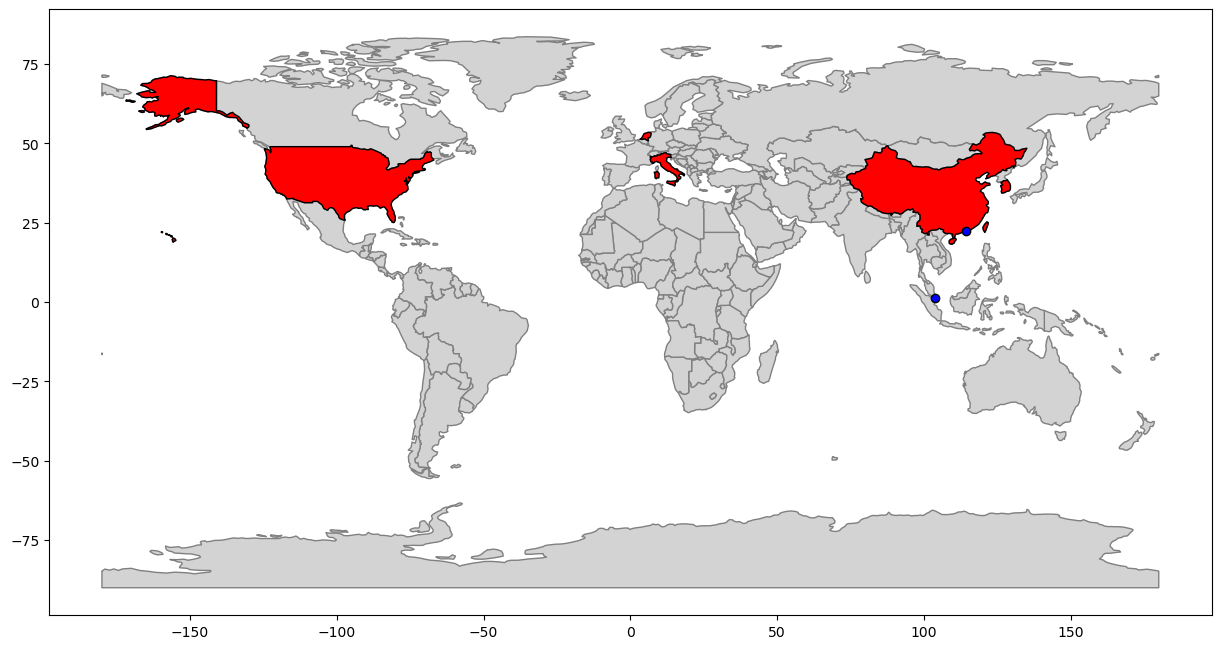
\includegraphics{Análisis_files/figure-pdf/fig-mapa-output-1.png}

}

\caption{\label{fig-mapa}Mapa con los lugares del que proceden las IPs}

\end{figure}

\begin{Shaded}
\begin{Highlighting}[]
\ImportTok{import}\NormalTok{ plotly.express }\ImportTok{as}\NormalTok{ px}
\end{Highlighting}
\end{Shaded}

\begin{Shaded}
\begin{Highlighting}[]
\ImportTok{import}\NormalTok{ seaborn }\ImportTok{as}\NormalTok{ sns}
\end{Highlighting}
\end{Shaded}

\begin{Shaded}
\begin{Highlighting}[]
\NormalTok{sns.}\BuiltInTok{set}\NormalTok{(style}\OperatorTok{=}\StringTok{\textquotesingle{}darkgrid\textquotesingle{}}\NormalTok{)}
\NormalTok{sns.countplot(data}\OperatorTok{=}\NormalTok{dfgdp, y}\OperatorTok{=}\StringTok{"codigoPais"}\NormalTok{)}
\NormalTok{ylabel }\OperatorTok{=}\NormalTok{ plt.ylabel(}\StringTok{"Pais"}\NormalTok{, rotation}\OperatorTok{=}\StringTok{\textquotesingle{}horizontal\textquotesingle{}}\NormalTok{)}
\NormalTok{plt.xlabel(}\StringTok{"Reportes"}\NormalTok{)}
\NormalTok{plt.show()}
\end{Highlighting}
\end{Shaded}

\begin{figure}[H]

{\centering 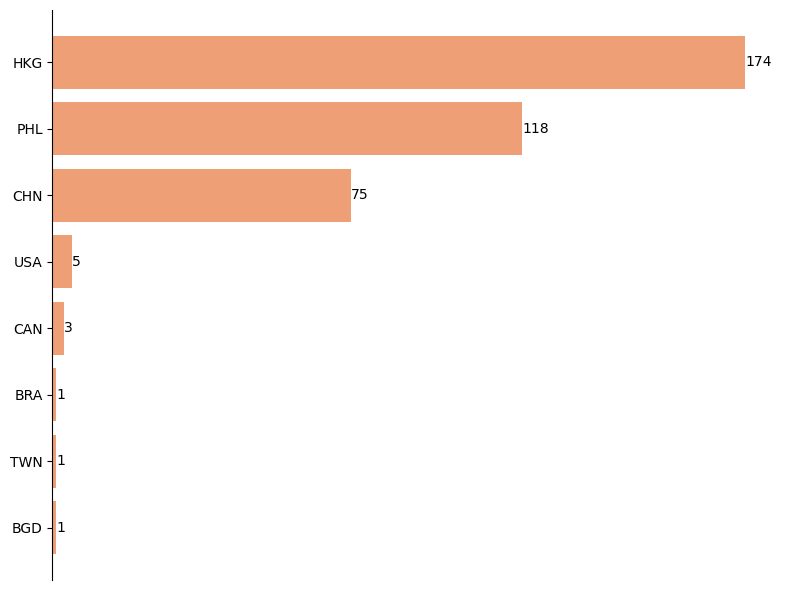
\includegraphics{Análisis_files/figure-pdf/fig-countplot-output-1.png}

}

\caption{\label{fig-countplot}Pais vs Nro de reportes}

\end{figure}

\begin{Shaded}
\begin{Highlighting}[]
\NormalTok{recuento }\OperatorTok{=}\NormalTok{ dfgdp[}\StringTok{"codigoPais"}\NormalTok{].value\_counts().to\_dict()}

\NormalTok{dfPlot }\OperatorTok{=}\NormalTok{ pd.DataFrame(data}\OperatorTok{=}\NormalTok{\{}\StringTok{"codigoPais"}\NormalTok{: }\BuiltInTok{list}\NormalTok{(recuento.keys()), }\StringTok{"Reportes"}\NormalTok{: }\BuiltInTok{list}\NormalTok{(recuento.values())\})}
\NormalTok{dfPlot}

\NormalTok{fig }\OperatorTok{=}\NormalTok{ px.scatter\_geo(dfPlot, locations}\OperatorTok{=}\StringTok{"codigoPais"}\NormalTok{, color}\OperatorTok{=}\StringTok{"codigoPais"}\NormalTok{, size}\OperatorTok{=}\StringTok{"Reportes"}\NormalTok{,}
\NormalTok{                     projection}\OperatorTok{=}\StringTok{"equirectangular"}\NormalTok{)}
\NormalTok{fig.write\_image(}\StringTok{"data/plotlySSH.png"}\NormalTok{)}
\end{Highlighting}
\end{Shaded}

\begin{Shaded}
\begin{Highlighting}[]
\ImportTok{from}\NormalTok{ PIL }\ImportTok{import}\NormalTok{ Image }

\NormalTok{image }\OperatorTok{=}\NormalTok{ np.asarray(Image.}\BuiltInTok{open}\NormalTok{(}\StringTok{\textquotesingle{}data/plotlySSH.png\textquotesingle{}}\NormalTok{))}
\NormalTok{plt.imshow(image)}
\NormalTok{plt.grid(}\VariableTok{False}\NormalTok{)}
\NormalTok{plt.axis(}\VariableTok{False}\NormalTok{)}
\NormalTok{plt.show()}
\end{Highlighting}
\end{Shaded}

\begin{figure}[H]

{\centering 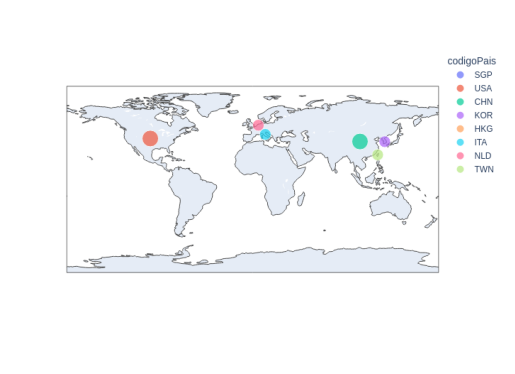
\includegraphics{Análisis_files/figure-pdf/fig-scatergeo-output-1.png}

}

\caption{\label{fig-scatergeo}Scatterplot con tamaño en función de
número de reportes}

\end{figure}

\begin{Shaded}
\begin{Highlighting}[]
\NormalTok{recuento }\OperatorTok{=}\NormalTok{ df[}\StringTok{"pais"}\NormalTok{].value\_counts().to\_dict()}

\NormalTok{pd.DataFrame(data}\OperatorTok{=}\NormalTok{\{}\StringTok{"Pais"}\NormalTok{: }\BuiltInTok{list}\NormalTok{(recuento.keys()), }\StringTok{"Reportes"}\NormalTok{: }\BuiltInTok{list}\NormalTok{(recuento.values())\})}
\end{Highlighting}
\end{Shaded}

\begin{longtable}[]{@{}lll@{}}
\toprule\noalign{}
& Pais & Reportes \\
\midrule\noalign{}
\endhead
\bottomrule\noalign{}
\endlastfoot
0 & Singapore & 3 \\
1 & United States & 2 \\
2 & China & 2 \\
3 & Korea, Republic of & 1 \\
4 & Hong Kong & 1 \\
5 & Italy & 1 \\
6 & Netherlands & 1 \\
7 & Taiwan, Province of China & 1 \\
\end{longtable}

\hypertarget{anuxe1lisis-de-frecuencia}{%
\subsubsection{Análisis de frecuencia}\label{anuxe1lisis-de-frecuencia}}

Para así poder de tratar de identificar cierto patron asociado a la hora
de ataque.

\hypertarget{extracciuxf3n-de-informaciuxf3n}{%
\paragraph{Extracción de
información}\label{extracciuxf3n-de-informaciuxf3n}}

\begin{Shaded}
\begin{Highlighting}[]
\NormalTok{patron }\OperatorTok{=} \StringTok{"[0{-}9]\{1,3\}\textbackslash{}.[0{-}9]\{1,3\}\textbackslash{}.[0{-}9]\{1,3\}\textbackslash{}.[0{-}9]\{1,3\}"}
\OperatorTok{!}\NormalTok{grep }\OperatorTok{{-}}\NormalTok{Eo }\StringTok{"$patron"}\NormalTok{ data}\OperatorTok{/}\NormalTok{SSH.txt }\OperatorTok{\textgreater{}}\NormalTok{ data}\OperatorTok{/}\NormalTok{IPsSSH.txt}

\NormalTok{patron }\OperatorTok{=} \StringTok{"[a{-}z]}\SpecialCharTok{\{3\}}\StringTok{\textbackslash{}/[0{-}9]}\SpecialCharTok{\{2\}}\StringTok{\textbackslash{}/[0{-}9]}\SpecialCharTok{\{4\}}\StringTok{"}
\OperatorTok{!}\NormalTok{grep }\OperatorTok{{-}}\NormalTok{Eo }\StringTok{"$patron"}\NormalTok{ data}\OperatorTok{/}\NormalTok{SSH.txt }\OperatorTok{\textgreater{}\textgreater{}}\NormalTok{ data}\OperatorTok{/}\NormalTok{IPsSSH.txt}

\NormalTok{patron }\OperatorTok{=} \StringTok{"[0{-}9]}\SpecialCharTok{\{2\}}\StringTok{\textbackslash{}:[0{-}9]}\SpecialCharTok{\{2\}}\StringTok{\textbackslash{}:[0{-}9]}\SpecialCharTok{\{2\}}\StringTok{"}
\OperatorTok{!}\NormalTok{grep }\OperatorTok{{-}}\NormalTok{Eo }\StringTok{"$patron"}\NormalTok{ data}\OperatorTok{/}\NormalTok{SSH.txt }\OperatorTok{\textgreater{}\textgreater{}}\NormalTok{ data}\OperatorTok{/}\NormalTok{IPsSSH.txt}
\end{Highlighting}
\end{Shaded}

\begin{Shaded}
\begin{Highlighting}[]
\ControlFlowTok{with} \BuiltInTok{open}\NormalTok{(}\StringTok{"data/IPsSSH.txt"}\NormalTok{) }\ImportTok{as}\NormalTok{ ips:}
\NormalTok{    data }\OperatorTok{=}\NormalTok{ ips.read()}
\NormalTok{    data }\OperatorTok{=}\NormalTok{ data.replace(}\StringTok{"}\CharTok{\textbackslash{}n}\StringTok{"}\NormalTok{, }\StringTok{" "}\NormalTok{).split()}
\end{Highlighting}
\end{Shaded}

\begin{Shaded}
\begin{Highlighting}[]
\ControlFlowTok{for}\NormalTok{ i }\KeywordTok{in} \BuiltInTok{range}\NormalTok{(}\BuiltInTok{int}\NormalTok{(}\BuiltInTok{len}\NormalTok{(data)}\OperatorTok{/}\DecValTok{3}\NormalTok{)):}
\NormalTok{    data[i] }\OperatorTok{=}\NormalTok{ data[i] }\OperatorTok{+} \StringTok{" "} \OperatorTok{+}\NormalTok{ data[}\BuiltInTok{int}\NormalTok{(}\BuiltInTok{len}\NormalTok{(data)}\OperatorTok{/}\DecValTok{3}\NormalTok{)}\OperatorTok{+}\NormalTok{i] }\OperatorTok{+} \StringTok{" "} \OperatorTok{+}\NormalTok{ data[(}\BuiltInTok{int}\NormalTok{(}\BuiltInTok{len}\NormalTok{(data)}\OperatorTok{/}\DecValTok{3}\NormalTok{))}\OperatorTok{*}\DecValTok{2}\OperatorTok{+}\NormalTok{i]}
    
\NormalTok{data }\OperatorTok{=}\NormalTok{ data[:}\BuiltInTok{int}\NormalTok{(}\BuiltInTok{len}\NormalTok{(data)}\OperatorTok{/}\DecValTok{3}\NormalTok{)]}
\end{Highlighting}
\end{Shaded}

\begin{Shaded}
\begin{Highlighting}[]
\ImportTok{from}\NormalTok{ datetime }\ImportTok{import}\NormalTok{ datetime, time}
\NormalTok{diccInfo }\OperatorTok{=}\NormalTok{ \{}
    \StringTok{"IP"}\NormalTok{: [],}
    \StringTok{"Fecha"}\NormalTok{: [],}
    \StringTok{"Hora"}\NormalTok{: []}
\NormalTok{\}}
\NormalTok{eventos }\OperatorTok{=}\NormalTok{ []}

\ControlFlowTok{for}\NormalTok{ i }\KeywordTok{in}\NormalTok{ data:}
\NormalTok{    diccInfo[}\StringTok{"IP"}\NormalTok{].append(i.split()[}\DecValTok{0}\NormalTok{])}
\NormalTok{    diccInfo[}\StringTok{"Fecha"}\NormalTok{].append(i.split()[}\DecValTok{1}\NormalTok{])}
\NormalTok{    mes }\OperatorTok{=} \DecValTok{5}
\NormalTok{    dia }\OperatorTok{=} \BuiltInTok{int}\NormalTok{(i.split()[}\DecValTok{1}\NormalTok{].split(sep}\OperatorTok{=}\StringTok{"/"}\NormalTok{)[}\DecValTok{1}\NormalTok{])}
\NormalTok{    año }\OperatorTok{=} \BuiltInTok{int}\NormalTok{(i.split()[}\DecValTok{1}\NormalTok{].split(sep}\OperatorTok{=}\StringTok{"/"}\NormalTok{)[}\DecValTok{2}\NormalTok{])}
\NormalTok{    h }\OperatorTok{=} \BuiltInTok{int}\NormalTok{(i.split()[}\DecValTok{2}\NormalTok{].split(sep}\OperatorTok{=}\StringTok{":"}\NormalTok{)[}\DecValTok{0}\NormalTok{])}
\NormalTok{    m }\OperatorTok{=} \BuiltInTok{int}\NormalTok{(i.split()[}\DecValTok{2}\NormalTok{].split(sep}\OperatorTok{=}\StringTok{":"}\NormalTok{)[}\DecValTok{1}\NormalTok{])}
\NormalTok{    s }\OperatorTok{=} \BuiltInTok{int}\NormalTok{(i.split()[}\DecValTok{2}\NormalTok{].split(sep}\OperatorTok{=}\StringTok{":"}\NormalTok{)[}\DecValTok{2}\NormalTok{])}
\NormalTok{    diccInfo[}\StringTok{"Hora"}\NormalTok{].append(time(hour}\OperatorTok{=}\BuiltInTok{int}\NormalTok{(h), minute}\OperatorTok{=}\BuiltInTok{int}\NormalTok{(m), second}\OperatorTok{=}\BuiltInTok{int}\NormalTok{(s)))}
    \CommentTok{\#diccInfo["Hora"].append(i.split()[2])}
    
\NormalTok{    eventos.append((i.split()[}\DecValTok{0}\NormalTok{],datetime(year}\OperatorTok{=}\NormalTok{año, month}\OperatorTok{=}\NormalTok{mes, day}\OperatorTok{=}\NormalTok{dia, hour}\OperatorTok{=}\NormalTok{h, minute}\OperatorTok{=}\NormalTok{m)))}
\end{Highlighting}
\end{Shaded}

\begin{Shaded}
\begin{Highlighting}[]
\NormalTok{dfHora }\OperatorTok{=}\NormalTok{ pd.DataFrame(data}\OperatorTok{=}\NormalTok{diccInfo)}
\end{Highlighting}
\end{Shaded}

\begin{Shaded}
\begin{Highlighting}[]
\NormalTok{dfHora[}\StringTok{"Pais"}\NormalTok{] }\OperatorTok{=} \VariableTok{None}
\ControlFlowTok{for}\NormalTok{ index, row }\KeywordTok{in}\NormalTok{ dfHora.iterrows():}
\NormalTok{    ip }\OperatorTok{=}\NormalTok{ row[}\StringTok{"IP"}\NormalTok{]}
\NormalTok{    row[}\StringTok{"Pais"}\NormalTok{] }\OperatorTok{=}\NormalTok{ df[df[}\StringTok{\textquotesingle{}ip\textquotesingle{}}\NormalTok{] }\OperatorTok{==}\NormalTok{ ip].iloc[}\DecValTok{0}\NormalTok{][}\StringTok{\textquotesingle{}pais\textquotesingle{}}\NormalTok{]}
\end{Highlighting}
\end{Shaded}

\begin{Shaded}
\begin{Highlighting}[]
\NormalTok{fig, ax }\OperatorTok{=}\NormalTok{ plt.subplots()}

\NormalTok{fecha }\OperatorTok{=}\NormalTok{ [evento[}\DecValTok{1}\NormalTok{] }\ControlFlowTok{for}\NormalTok{ evento }\KeywordTok{in}\NormalTok{ eventos]}
\NormalTok{etiquetas }\OperatorTok{=}\NormalTok{ [evento[}\DecValTok{0}\NormalTok{] }\ControlFlowTok{for}\NormalTok{ evento }\KeywordTok{in}\NormalTok{ eventos]}
\NormalTok{ax.eventplot(fecha, lineoffsets}\OperatorTok{=}\FloatTok{0.1}\NormalTok{, linelengths}\OperatorTok{=}\FloatTok{0.1}\NormalTok{, color}\OperatorTok{=}\StringTok{\textquotesingle{}r\textquotesingle{}}\NormalTok{)}
\NormalTok{ax.set\_ylabel(}\VariableTok{None}\NormalTok{)}
\NormalTok{ax.set\_yticklabels([])}
\NormalTok{ax.set\_xlim(datetime(}\DecValTok{2023}\NormalTok{, }\DecValTok{5}\NormalTok{, }\DecValTok{23}\NormalTok{, }\DecValTok{0}\NormalTok{, }\DecValTok{0}\NormalTok{), datetime(}\DecValTok{2023}\NormalTok{, }\DecValTok{5}\NormalTok{, }\DecValTok{23}\NormalTok{, }\DecValTok{23}\NormalTok{, }\DecValTok{59}\NormalTok{))}
\NormalTok{fig.autofmt\_xdate()}
\end{Highlighting}
\end{Shaded}

\begin{figure}[H]

{\centering 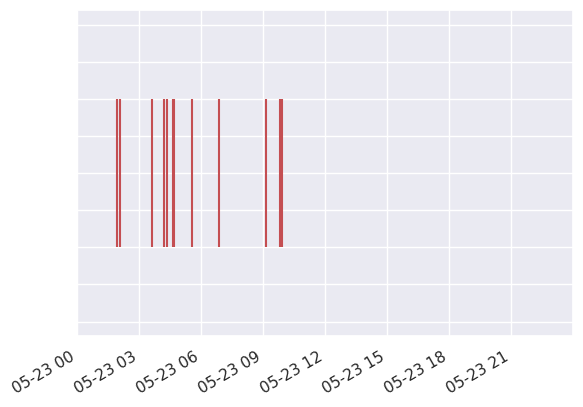
\includegraphics{Análisis_files/figure-pdf/fig-eventos-output-1.png}

}

\caption{\label{fig-eventos}Visualización de eventos de SSH}

\end{figure}

\hypertarget{anuxe1lisis-de-isps}{%
\subsubsection{Análisis de ISPs}\label{anuxe1lisis-de-isps}}

\begin{Shaded}
\begin{Highlighting}[]
\NormalTok{recuento }\OperatorTok{=}\NormalTok{ df[}\StringTok{"isp"}\NormalTok{].value\_counts().to\_dict()}

\NormalTok{recuento }\OperatorTok{=}\NormalTok{ pd.DataFrame(data}\OperatorTok{=}\NormalTok{\{}\StringTok{"ISP"}\NormalTok{: }\BuiltInTok{list}\NormalTok{(recuento.keys()), }\StringTok{"Reportes"}\NormalTok{: }\BuiltInTok{list}\NormalTok{(recuento.values())\})}
\NormalTok{recuento}
\end{Highlighting}
\end{Shaded}

\begin{longtable}[]{@{}lll@{}}
\toprule\noalign{}
& ISP & Reportes \\
\midrule\noalign{}
\endhead
\bottomrule\noalign{}
\endlastfoot
0 & DigitalOcean LLC & 3 \\
1 & ChinaNet Jiangsu Province Network & 2 \\
2 & Amazon Data Services NoVa & 1 \\
3 & KT Corporation & 1 \\
4 & Pacswitch Globe Telecom Limited & 1 \\
5 & Vodafone Italia S.p.A. & 1 \\
6 & FiberXpress BV & 1 \\
7 & Alibaba.com Singapore E-Commerce Private Limited & 1 \\
8 & Chunghwa Telecom Co. Ltd. & 1 \\
\end{longtable}

\begin{Shaded}
\begin{Highlighting}[]
\NormalTok{fig}\OperatorTok{=}\NormalTok{plt.plot(figsize}\OperatorTok{=}\NormalTok{(}\DecValTok{15}\NormalTok{, }\DecValTok{10}\NormalTok{))}
\NormalTok{sns.countplot(data}\OperatorTok{=}\NormalTok{df, y}\OperatorTok{=}\StringTok{"isp"}\NormalTok{)}
\NormalTok{plt.tick\_params(labelsize }\OperatorTok{=} \DecValTok{11}\NormalTok{)}
\NormalTok{plt.xticks([}\DecValTok{1}\NormalTok{,}\DecValTok{2}\NormalTok{,}\DecValTok{3}\NormalTok{])}
\NormalTok{plt.ylabel(}\StringTok{"ISPs"}\NormalTok{, rotation}\OperatorTok{=}\DecValTok{0}\NormalTok{)}
\NormalTok{plt.xlabel(}\StringTok{"Veces denunciado"}\NormalTok{)}
\NormalTok{plt.show()}
\end{Highlighting}
\end{Shaded}

\begin{figure}[H]

{\centering 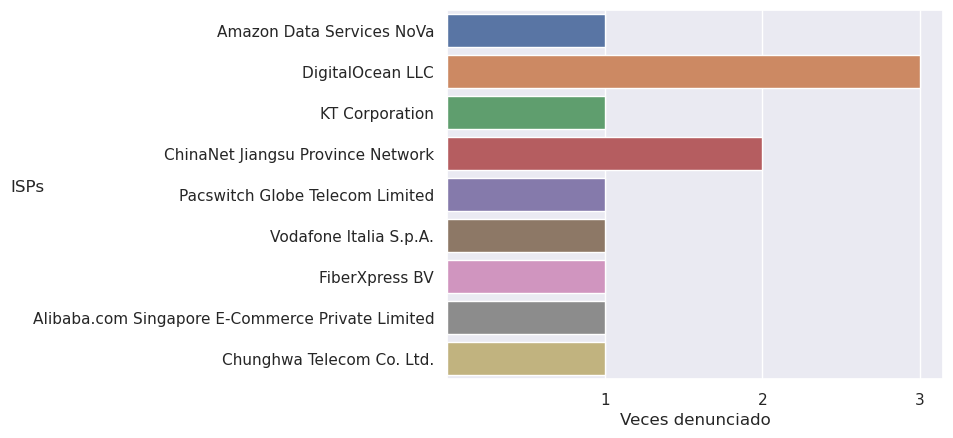
\includegraphics{Análisis_files/figure-pdf/fig-isps-output-1.png}

}

\caption{\label{fig-isps}Número de veces que se denuncio un ISp}

\end{figure}

\hypertarget{anuxe1lisis-de-uso}{%
\subsubsection{Análisis de uso}\label{anuxe1lisis-de-uso}}

\begin{Shaded}
\begin{Highlighting}[]
\NormalTok{recuento }\OperatorTok{=}\NormalTok{ df[}\StringTok{"tipoDeUso"}\NormalTok{].value\_counts().to\_dict()}

\NormalTok{recuento }\OperatorTok{=}\NormalTok{ pd.DataFrame(data}\OperatorTok{=}\NormalTok{\{}\StringTok{"uso"}\NormalTok{: }\BuiltInTok{list}\NormalTok{(recuento.keys()), }\StringTok{"Reportes"}\NormalTok{: }\BuiltInTok{list}\NormalTok{(recuento.values())\})}
\NormalTok{recuento}
\end{Highlighting}
\end{Shaded}

\begin{longtable}[]{@{}lll@{}}
\toprule\noalign{}
& uso & Reportes \\
\midrule\noalign{}
\endhead
\bottomrule\noalign{}
\endlastfoot
0 & Data Center/Web Hosting/Transit & 8 \\
1 & Fixed Line ISP & 1 \\
\end{longtable}

\begin{Shaded}
\begin{Highlighting}[]
\NormalTok{fig}\OperatorTok{=}\NormalTok{plt.plot(figsize}\OperatorTok{=}\NormalTok{(}\DecValTok{15}\NormalTok{, }\DecValTok{10}\NormalTok{))}
\NormalTok{sns.countplot(data}\OperatorTok{=}\NormalTok{df, y}\OperatorTok{=}\StringTok{"tipoDeUso"}\NormalTok{)}
\NormalTok{plt.tick\_params(labelsize }\OperatorTok{=} \DecValTok{11}\NormalTok{)}
\CommentTok{\#plt.xticks([1,2,3])}
\NormalTok{plt.ylabel(}\StringTok{"Tipo de uso"}\NormalTok{, rotation}\OperatorTok{=}\DecValTok{0}\NormalTok{)}
\NormalTok{plt.xlabel(}\StringTok{"Nro de IPs"}\NormalTok{)}
\NormalTok{plt.show()}
\end{Highlighting}
\end{Shaded}

\begin{figure}[H]

{\centering 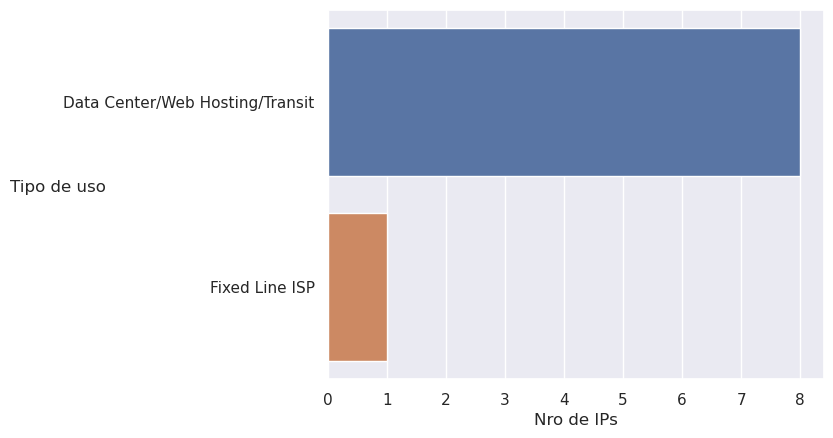
\includegraphics{Análisis_files/figure-pdf/fig-tipodeusossh-output-1.png}

}

\caption{\label{fig-tipodeusossh}Tipo de uso declarado por las IPs}

\end{figure}

\hypertarget{anuxe1lisis-de-ips-reportadas-por-ataque-ddos}{%
\subsection{Análisis de IPs reportadas por ataque
DDoS}\label{anuxe1lisis-de-ips-reportadas-por-ataque-ddos}}

\hypertarget{extracciuxf3n-de-informaciuxf3n-1}{%
\subsubsection{Extracción de
información}\label{extracciuxf3n-de-informaciuxf3n-1}}

\begin{Shaded}
\begin{Highlighting}[]
\NormalTok{patron }\OperatorTok{=} \StringTok{"[0{-}9]\{1,3\}\textbackslash{}.[0{-}9]\{1,3\}\textbackslash{}.[0{-}9]\{1,3\}\textbackslash{}.[0{-}9]\{1,3\}"}
\OperatorTok{!}\NormalTok{grep }\OperatorTok{{-}}\NormalTok{Eo }\StringTok{"$patron"}\NormalTok{ data}\OperatorTok{/}\NormalTok{DDOS.txt }\OperatorTok{\textgreater{}}\NormalTok{ data}\OperatorTok{/}\NormalTok{IPsDDoS.txt}

\NormalTok{patron }\OperatorTok{=} \StringTok{"[a{-}z]}\SpecialCharTok{\{3\}}\StringTok{\textbackslash{}/[0{-}9]}\SpecialCharTok{\{2\}}\StringTok{\textbackslash{}/[0{-}9]}\SpecialCharTok{\{4\}}\StringTok{"}
\OperatorTok{!}\NormalTok{grep }\OperatorTok{{-}}\NormalTok{Eo }\StringTok{"$patron"}\NormalTok{ data}\OperatorTok{/}\NormalTok{DDOS.txt }\OperatorTok{\textgreater{}\textgreater{}}\NormalTok{ data}\OperatorTok{/}\NormalTok{IPsDDoS.txt}

\NormalTok{patron }\OperatorTok{=} \StringTok{"[0{-}9]}\SpecialCharTok{\{2\}}\StringTok{\textbackslash{}:[0{-}9]}\SpecialCharTok{\{2\}}\StringTok{\textbackslash{}:[0{-}9]}\SpecialCharTok{\{2\}}\StringTok{"}
\OperatorTok{!}\NormalTok{grep }\OperatorTok{{-}}\NormalTok{Eo }\StringTok{"$patron"}\NormalTok{ data}\OperatorTok{/}\NormalTok{DDOS.txt }\OperatorTok{\textgreater{}\textgreater{}}\NormalTok{ data}\OperatorTok{/}\NormalTok{IPsDDoS.txt}
\end{Highlighting}
\end{Shaded}

\begin{Shaded}
\begin{Highlighting}[]
\ControlFlowTok{with} \BuiltInTok{open}\NormalTok{(}\StringTok{"data/IPsDDoS.txt"}\NormalTok{) }\ImportTok{as}\NormalTok{ ips:}
\NormalTok{    data }\OperatorTok{=}\NormalTok{ ips.read()}
\NormalTok{    data }\OperatorTok{=}\NormalTok{ data.replace(}\StringTok{"}\CharTok{\textbackslash{}n}\StringTok{"}\NormalTok{, }\StringTok{" "}\NormalTok{).split()}
\end{Highlighting}
\end{Shaded}

\begin{Shaded}
\begin{Highlighting}[]
\NormalTok{ips }\OperatorTok{=}\NormalTok{ []}
\NormalTok{dia }\OperatorTok{=}\NormalTok{ []}
\NormalTok{hora }\OperatorTok{=}\NormalTok{ []}
\ControlFlowTok{for}\NormalTok{ i }\KeywordTok{in} \BuiltInTok{range}\NormalTok{(}\BuiltInTok{int}\NormalTok{(}\BuiltInTok{len}\NormalTok{(data)}\OperatorTok{/}\DecValTok{3}\NormalTok{)):}
\NormalTok{    ips.append(data[i])}
\NormalTok{    dia.append(data[}\BuiltInTok{int}\NormalTok{(}\BuiltInTok{len}\NormalTok{(data)}\OperatorTok{/}\DecValTok{3}\NormalTok{)}\OperatorTok{+}\NormalTok{i])}
\NormalTok{    hora.append(data[(}\BuiltInTok{int}\NormalTok{(}\BuiltInTok{len}\NormalTok{(data)}\OperatorTok{/}\DecValTok{3}\NormalTok{))}\OperatorTok{*}\DecValTok{2}\OperatorTok{+}\NormalTok{i])}
\NormalTok{    data[i] }\OperatorTok{=}\NormalTok{ data[i] }\OperatorTok{+} \StringTok{" "} \OperatorTok{+}\NormalTok{ data[}\BuiltInTok{int}\NormalTok{(}\BuiltInTok{len}\NormalTok{(data)}\OperatorTok{/}\DecValTok{3}\NormalTok{)}\OperatorTok{+}\NormalTok{i] }\OperatorTok{+} \StringTok{" "} \OperatorTok{+}\NormalTok{ data[(}\BuiltInTok{int}\NormalTok{(}\BuiltInTok{len}\NormalTok{(data)}\OperatorTok{/}\DecValTok{3}\NormalTok{))}\OperatorTok{*}\DecValTok{2}\OperatorTok{+}\NormalTok{i]}
\end{Highlighting}
\end{Shaded}

\begin{Shaded}
\begin{Highlighting}[]
\NormalTok{data }\OperatorTok{=}\NormalTok{ data[:}\BuiltInTok{int}\NormalTok{(}\BuiltInTok{len}\NormalTok{(data)}\OperatorTok{/}\DecValTok{3}\NormalTok{)]}
\end{Highlighting}
\end{Shaded}

\begin{Shaded}
\begin{Highlighting}[]
\NormalTok{data }\OperatorTok{=}\NormalTok{ pd.DataFrame(data}\OperatorTok{=}\NormalTok{\{}\StringTok{\textquotesingle{}ip\textquotesingle{}}\NormalTok{: ips,}
                       \StringTok{\textquotesingle{}dia\textquotesingle{}}\NormalTok{: dia,}
                       \StringTok{\textquotesingle{}hora\textquotesingle{}}\NormalTok{: hora\})}
\end{Highlighting}
\end{Shaded}

\begin{Shaded}
\begin{Highlighting}[]
\NormalTok{apiAbuse }\OperatorTok{=}\NormalTok{ AbuseIPDB()}
\end{Highlighting}
\end{Shaded}

\begin{Shaded}
\begin{Highlighting}[]
\ImportTok{from}\NormalTok{ IPython.display }\ImportTok{import}\NormalTok{ clear\_output}
\CommentTok{\#Declaro las keys de la info que devuelve mi implementación de requests}
\NormalTok{keys }\OperatorTok{=}\NormalTok{ [}\StringTok{\textquotesingle{}esPublica\textquotesingle{}}\NormalTok{, }\StringTok{\textquotesingle{}estaEnWhitelist\textquotesingle{}}\NormalTok{, }\StringTok{\textquotesingle{}scoreAbuso\textquotesingle{}}\NormalTok{, }\StringTok{\textquotesingle{}pais\textquotesingle{}}\NormalTok{, }\StringTok{\textquotesingle{}codigoPais\textquotesingle{}}\NormalTok{, }\StringTok{\textquotesingle{}isp\textquotesingle{}}\NormalTok{, }\StringTok{\textquotesingle{}tipoDeUso\textquotesingle{}}\NormalTok{, }\StringTok{\textquotesingle{}ultimoReporte\textquotesingle{}}\NormalTok{]}

\NormalTok{diccDf }\OperatorTok{=}\NormalTok{ \{}\StringTok{\textquotesingle{}ip\textquotesingle{}}\NormalTok{ : []\}}

\ControlFlowTok{if}\NormalTok{ os.path.isfile(}\StringTok{"data/ipDDOS.csv"}\NormalTok{):}
    
\NormalTok{    df }\OperatorTok{=}\NormalTok{ pd.read\_csv(}\StringTok{"data/ipDDOS.csv"}\NormalTok{)}
    
\ControlFlowTok{else}\NormalTok{:}
    \ControlFlowTok{for}\NormalTok{ ip, i }\KeywordTok{in} \BuiltInTok{zip}\NormalTok{(ips, }\BuiltInTok{range}\NormalTok{(}\BuiltInTok{len}\NormalTok{(ips))):}
\NormalTok{        clear\_output()}
        \BuiltInTok{print}\NormalTok{(}\SpecialStringTok{f"}\SpecialCharTok{\{}\NormalTok{i}\SpecialCharTok{\}}\SpecialStringTok{/}\SpecialCharTok{\{}\BuiltInTok{len}\NormalTok{(ips)}\SpecialCharTok{\}}\SpecialStringTok{"}\NormalTok{)}
\NormalTok{        diccDf[}\StringTok{\textquotesingle{}ip\textquotesingle{}}\NormalTok{].append(ip)}
\NormalTok{        info }\OperatorTok{=}\NormalTok{ apiAbuse.getInfo(ip)}
        \ControlFlowTok{for}\NormalTok{ key }\KeywordTok{in}\NormalTok{ keys:}
            \ControlFlowTok{if}\NormalTok{ key }\KeywordTok{in}\NormalTok{ diccDf:}
\NormalTok{                diccDf[key].append(info[key])}
            \ControlFlowTok{else}\NormalTok{:}
\NormalTok{                diccDf[key] }\OperatorTok{=}\NormalTok{ [info[key]]}

\NormalTok{    df }\OperatorTok{=}\NormalTok{ pd.DataFrame(data}\OperatorTok{=}\NormalTok{diccDf)}
    
    
\NormalTok{df[}\StringTok{"hora"}\NormalTok{] }\OperatorTok{=}\NormalTok{ data[}\StringTok{"hora"}\NormalTok{]}
\NormalTok{df[}\StringTok{"dia"}\NormalTok{] }\OperatorTok{=}\NormalTok{ data[}\StringTok{"dia"}\NormalTok{]}
\end{Highlighting}
\end{Shaded}

\begin{verbatim}
377/378
\end{verbatim}

\begin{Shaded}
\begin{Highlighting}[]
\NormalTok{df}
\end{Highlighting}
\end{Shaded}

\begin{longtable}[]{@{}llllllllllll@{}}
\toprule\noalign{}
& ip & esPublica & estaEnWhitelist & scoreAbuso & pais & codigoPais &
isp & tipoDeUso & ultimoReporte & hora & dia \\
\midrule\noalign{}
\endhead
\bottomrule\noalign{}
\endlastfoot
0 & 45.204.126.117 & True & None & 0 & NaN & HK & Intercontinental
Internet Data Corp & Data Center/Web Hosting/Transit & None & 23:47:10 &
may/22/2023 \\
1 & 59.153.100.70 & True & None & 0 & NaN & BD & Dot Internet & Fixed
Line ISP & None & 23:47:10 & may/22/2023 \\
2 & 1.32.249.141 & True & None & 0 & NaN & HK & CTG Server Ltd. & Data
Center/Web Hosting/Transit & None & 23:47:10 & may/22/2023 \\
3 & 103.116.15.134 & True & None & 0 & NaN & TW & Shine Telecom Co. Ltd.
& Commercial & None & 23:47:10 & may/22/2023 \\
4 & 43.225.58.180 & True & None & 0 & NaN & HK & Dragon Spirit
Investments International Co. Li... & Data Center/Web Hosting/Transit &
None & 23:47:10 & may/22/2023 \\
... & ... & ... & ... & ... & ... & ... & ... & ... & ... & ... & ... \\
373 & 43.225.58.251 & True & None & 0 & NaN & HK & Dragon Spirit
Investments International Co. Li... & Data Center/Web Hosting/Transit &
None & 23:47:19 & may/22/2023 \\
374 & 43.225.58.88 & True & None & 0 & NaN & HK & Dragon Spirit
Investments International Co. Li... & Data Center/Web Hosting/Transit &
None & 23:47:19 & may/22/2023 \\
375 & 43.225.58.182 & True & None & 0 & NaN & HK & Dragon Spirit
Investments International Co. Li... & Data Center/Web Hosting/Transit &
None & 23:47:19 & may/22/2023 \\
376 & 103.119.129.64 & True & None & 0 & NaN & HK & Suniway Group
Limited & Data Center/Web Hosting/Transit & None & 23:47:19 &
may/22/2023 \\
377 & 43.225.58.19 & True & None & 0 & NaN & HK & Dragon Spirit
Investments International Co. Li... & Data Center/Web Hosting/Transit &
None & 23:47:19 & may/22/2023 \\
\end{longtable}

\begin{Shaded}
\begin{Highlighting}[]
\NormalTok{unameds }\OperatorTok{=}\NormalTok{ [i }\ControlFlowTok{for}\NormalTok{ i }\KeywordTok{in}\NormalTok{ df.columns }\ControlFlowTok{if} \StringTok{\textquotesingle{}Unnamed\textquotesingle{}} \KeywordTok{in}\NormalTok{ i]}
\ControlFlowTok{for}\NormalTok{ i }\KeywordTok{in}\NormalTok{ unameds:}
\NormalTok{    df.drop(i, axis}\OperatorTok{=}\DecValTok{1}\NormalTok{, inplace}\OperatorTok{=}\VariableTok{True}\NormalTok{)}
    
\NormalTok{df.to\_csv(}\StringTok{"data/ipDDOS.csv"}\NormalTok{, index}\OperatorTok{=}\VariableTok{False}\NormalTok{)}
\end{Highlighting}
\end{Shaded}

\hypertarget{uxedndices-de-abuso-1}{%
\subsubsection{Índices de abuso}\label{uxedndices-de-abuso-1}}

\begin{Shaded}
\begin{Highlighting}[]
\NormalTok{recuento }\OperatorTok{=}\NormalTok{ df[}\StringTok{"scoreAbuso"}\NormalTok{].value\_counts().to\_dict()}

\NormalTok{pd.DataFrame(data}\OperatorTok{=}\NormalTok{\{}\StringTok{"Pais"}\NormalTok{: }\BuiltInTok{list}\NormalTok{(recuento.keys()), }\StringTok{"Reportes"}\NormalTok{: }\BuiltInTok{list}\NormalTok{(recuento.values())\})}
\end{Highlighting}
\end{Shaded}

\begin{longtable}[]{@{}lll@{}}
\toprule\noalign{}
& Pais & Reportes \\
\midrule\noalign{}
\endhead
\bottomrule\noalign{}
\endlastfoot
0 & 0 & 375 \\
1 & 2 & 2 \\
2 & 10 & 1 \\
\end{longtable}

\hypertarget{anuxe1lisis-de-procedencia-1}{%
\subsubsection{Análisis de
procedencia}\label{anuxe1lisis-de-procedencia-1}}

\begin{Shaded}
\begin{Highlighting}[]
\ImportTok{import}\NormalTok{ pycountry}
\end{Highlighting}
\end{Shaded}

\begin{Shaded}
\begin{Highlighting}[]
\NormalTok{df[}\StringTok{\textquotesingle{}pais\textquotesingle{}}\NormalTok{] }\OperatorTok{=}\NormalTok{ df[}\StringTok{\textquotesingle{}codigoPais\textquotesingle{}}\NormalTok{].}\BuiltInTok{apply}\NormalTok{(}\KeywordTok{lambda}\NormalTok{ codigo: pycountry.countries.get(alpha\_2}\OperatorTok{=}\NormalTok{codigo).name)}
\NormalTok{dfgdp }\OperatorTok{=}\NormalTok{ df.copy()}
\NormalTok{dfgdp[}\StringTok{\textquotesingle{}codigoPais\textquotesingle{}}\NormalTok{] }\OperatorTok{=}\NormalTok{ df[}\StringTok{\textquotesingle{}pais\textquotesingle{}}\NormalTok{].}\BuiltInTok{apply}\NormalTok{(}\KeywordTok{lambda}\NormalTok{ nombre: pycountry.countries.search\_fuzzy(nombre)[}\DecValTok{0}\NormalTok{].alpha\_3)}
\end{Highlighting}
\end{Shaded}

\begin{Shaded}
\begin{Highlighting}[]
\ImportTok{import}\NormalTok{ geopandas }\ImportTok{as}\NormalTok{ gpd}
\ImportTok{import}\NormalTok{ matplotlib.pyplot }\ImportTok{as}\NormalTok{ plt}

\NormalTok{mapa }\OperatorTok{=}\NormalTok{ gpd.read\_file(gpd.datasets.get\_path(}\StringTok{\textquotesingle{}naturalearth\_lowres\textquotesingle{}}\NormalTok{))}
\end{Highlighting}
\end{Shaded}

\begin{Shaded}
\begin{Highlighting}[]
\BuiltInTok{print}\NormalTok{(np.unique(dfgdp[}\StringTok{"codigoPais"}\NormalTok{].loc[}\OperatorTok{\textasciitilde{}}\NormalTok{dfgdp[}\StringTok{"codigoPais"}\NormalTok{].isin(mapa[}\StringTok{"iso\_a3"}\NormalTok{])]))}
\end{Highlighting}
\end{Shaded}

\begin{verbatim}
['HKG']
\end{verbatim}

\begin{Shaded}
\begin{Highlighting}[]
\NormalTok{paisesMarcados }\OperatorTok{=}\NormalTok{ mapa[mapa[}\StringTok{\textquotesingle{}iso\_a3\textquotesingle{}}\NormalTok{].isin(dfgdp[}\StringTok{"codigoPais"}\NormalTok{])]}

\NormalTok{fig, ax }\OperatorTok{=}\NormalTok{ plt.subplots(figsize}\OperatorTok{=}\NormalTok{(}\DecValTok{15}\NormalTok{, }\DecValTok{10}\NormalTok{))}

\NormalTok{mapa.plot(ax}\OperatorTok{=}\NormalTok{ax, edgecolor}\OperatorTok{=}\StringTok{\textquotesingle{}grey\textquotesingle{}}\NormalTok{, color}\OperatorTok{=}\StringTok{\textquotesingle{}lightgrey\textquotesingle{}}\NormalTok{)}
\NormalTok{paisesMarcados.plot(ax}\OperatorTok{=}\NormalTok{ax, edgecolor}\OperatorTok{=}\StringTok{\textquotesingle{}black\textquotesingle{}}\NormalTok{, color}\OperatorTok{=}\StringTok{\textquotesingle{}red\textquotesingle{}}\NormalTok{)}

\NormalTok{ciudades }\OperatorTok{=}\NormalTok{ gpd.read\_file(gpd.datasets.get\_path(}\StringTok{\textquotesingle{}naturalearth\_cities\textquotesingle{}}\NormalTok{))}

\NormalTok{hongkong }\OperatorTok{=}\NormalTok{ ciudades[ciudades[}\StringTok{\textquotesingle{}name\textquotesingle{}}\NormalTok{] }\OperatorTok{==} \StringTok{\textquotesingle{}Hong Kong\textquotesingle{}}\NormalTok{]}

\NormalTok{hongkong.plot(ax}\OperatorTok{=}\NormalTok{ax, edgecolor}\OperatorTok{=}\StringTok{\textquotesingle{}black\textquotesingle{}}\NormalTok{, color}\OperatorTok{=}\StringTok{\textquotesingle{}blue\textquotesingle{}}\NormalTok{)}

\NormalTok{plt.show()}
\end{Highlighting}
\end{Shaded}

\begin{figure}[H]

{\centering 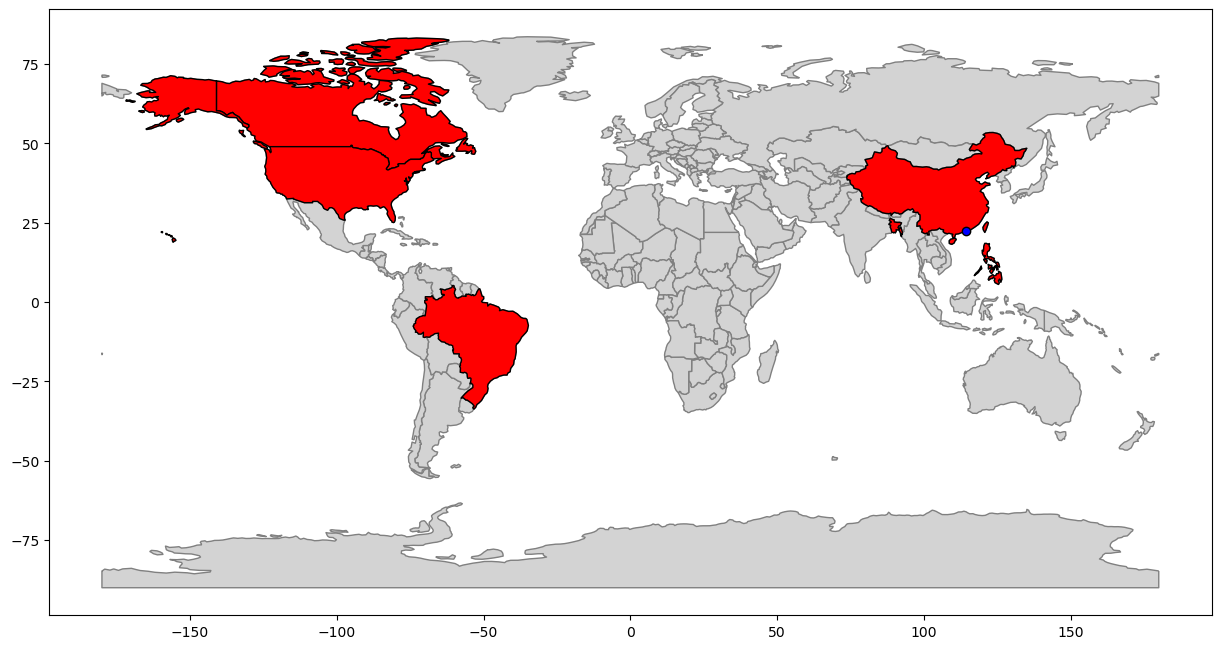
\includegraphics{Análisis_files/figure-pdf/fig-mapaddos-output-1.png}

}

\caption{\label{fig-mapaddos}Mapa con los lugares del que proceden las
IPs}

\end{figure}

\begin{Shaded}
\begin{Highlighting}[]
\NormalTok{recuento }\OperatorTok{=}\NormalTok{ df[}\StringTok{"pais"}\NormalTok{].value\_counts().to\_dict()}

\NormalTok{pd.DataFrame(data}\OperatorTok{=}\NormalTok{\{}\StringTok{"Pais"}\NormalTok{: }\BuiltInTok{list}\NormalTok{(recuento.keys()), }\StringTok{"Reportes"}\NormalTok{: }\BuiltInTok{list}\NormalTok{(recuento.values())\})}
\end{Highlighting}
\end{Shaded}

\begin{longtable}[]{@{}lll@{}}
\toprule\noalign{}
& Pais & Reportes \\
\midrule\noalign{}
\endhead
\bottomrule\noalign{}
\endlastfoot
0 & Hong Kong & 174 \\
1 & Philippines & 118 \\
2 & China & 75 \\
3 & United States & 5 \\
4 & Canada & 3 \\
5 & Bangladesh & 1 \\
6 & Taiwan, Province of China & 1 \\
7 & Brazil & 1 \\
\end{longtable}

\begin{Shaded}
\begin{Highlighting}[]
\NormalTok{sns.}\BuiltInTok{set}\NormalTok{(style}\OperatorTok{=}\StringTok{\textquotesingle{}darkgrid\textquotesingle{}}\NormalTok{)}
\NormalTok{sns.countplot(data}\OperatorTok{=}\NormalTok{dfgdp, y}\OperatorTok{=}\StringTok{"codigoPais"}\NormalTok{)}
\NormalTok{ylabel }\OperatorTok{=}\NormalTok{ plt.ylabel(}\StringTok{"Pais"}\NormalTok{, rotation}\OperatorTok{=}\StringTok{\textquotesingle{}horizontal\textquotesingle{}}\NormalTok{)}
\NormalTok{plt.xlabel(}\StringTok{"Reportes"}\NormalTok{)}
\NormalTok{plt.show()}
\end{Highlighting}
\end{Shaded}

\begin{figure}[H]

{\centering 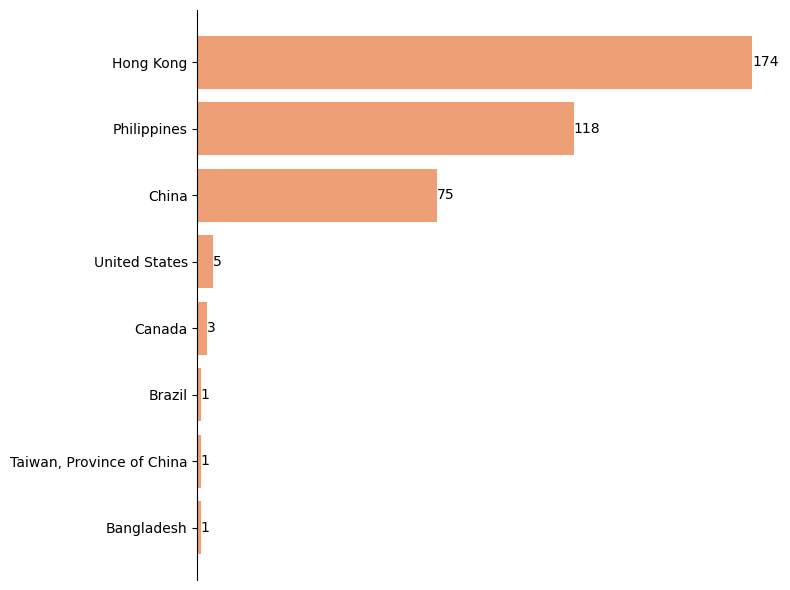
\includegraphics{Análisis_files/figure-pdf/fig-countplotddos-output-1.png}

}

\caption{\label{fig-countplotddos}Pais vs Nro de reportes}

\end{figure}

\begin{Shaded}
\begin{Highlighting}[]
\NormalTok{recuento }\OperatorTok{=}\NormalTok{ dfgdp[}\StringTok{"codigoPais"}\NormalTok{].value\_counts().to\_dict()}

\NormalTok{dfPlot }\OperatorTok{=}\NormalTok{ pd.DataFrame(data}\OperatorTok{=}\NormalTok{\{}\StringTok{"codigoPais"}\NormalTok{: }\BuiltInTok{list}\NormalTok{(recuento.keys()), }\StringTok{"Reportes"}\NormalTok{: }\BuiltInTok{list}\NormalTok{(recuento.values())\})}
\NormalTok{dfPlot}

\NormalTok{fig }\OperatorTok{=}\NormalTok{ px.scatter\_geo(dfPlot, locations}\OperatorTok{=}\StringTok{"codigoPais"}\NormalTok{, color}\OperatorTok{=}\StringTok{"codigoPais"}\NormalTok{, size}\OperatorTok{=}\StringTok{"Reportes"}\NormalTok{,}
\NormalTok{                     projection}\OperatorTok{=}\StringTok{"equirectangular"}\NormalTok{)}
\NormalTok{fig.write\_image(}\StringTok{"data/plotlyDDoS.png"}\NormalTok{)}
\end{Highlighting}
\end{Shaded}

\begin{Shaded}
\begin{Highlighting}[]
\ImportTok{from}\NormalTok{ PIL }\ImportTok{import}\NormalTok{ Image }

\NormalTok{image }\OperatorTok{=}\NormalTok{ np.asarray(Image.}\BuiltInTok{open}\NormalTok{(}\StringTok{\textquotesingle{}data/plotlyDDoS.png\textquotesingle{}}\NormalTok{))}
\NormalTok{plt.imshow(image)}
\NormalTok{plt.grid(}\VariableTok{False}\NormalTok{)}
\NormalTok{plt.axis(}\VariableTok{False}\NormalTok{)}
\NormalTok{plt.show()}
\end{Highlighting}
\end{Shaded}

\begin{figure}[H]

{\centering 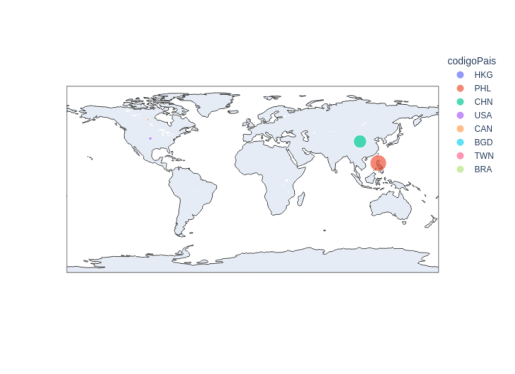
\includegraphics{Análisis_files/figure-pdf/fig-scatergeoddos-output-1.png}

}

\caption{\label{fig-scatergeoddos}Scatterplot con tamaño en función de
número de reportes}

\end{figure}

\hypertarget{anuxe1lisis-de-frecuencia-1}{%
\subsubsection{Análisis de
frecuencia}\label{anuxe1lisis-de-frecuencia-1}}

Para así poder de tratar de identificar cierto patron asociado a la hora
de ataque.

\hypertarget{extracciuxf3n-de-informaciuxf3n-2}{%
\paragraph{Extracción de
información}\label{extracciuxf3n-de-informaciuxf3n-2}}

\begin{Shaded}
\begin{Highlighting}[]
\NormalTok{df.head(}\DecValTok{3}\NormalTok{)}
\end{Highlighting}
\end{Shaded}

\begin{longtable}[]{@{}llllllllllll@{}}
\toprule\noalign{}
& ip & esPublica & estaEnWhitelist & scoreAbuso & pais & codigoPais &
isp & tipoDeUso & ultimoReporte & hora & dia \\
\midrule\noalign{}
\endhead
\bottomrule\noalign{}
\endlastfoot
0 & 45.204.126.117 & True & None & 0 & Hong Kong & HK & Intercontinental
Internet Data Corp & Data Center/Web Hosting/Transit & None & 23:47:10 &
may/22/2023 \\
1 & 59.153.100.70 & True & None & 0 & Bangladesh & BD & Dot Internet &
Fixed Line ISP & None & 23:47:10 & may/22/2023 \\
2 & 1.32.249.141 & True & None & 0 & Hong Kong & HK & CTG Server Ltd. &
Data Center/Web Hosting/Transit & None & 23:47:10 & may/22/2023 \\
\end{longtable}

\begin{Shaded}
\begin{Highlighting}[]
\NormalTok{eventosDDoS }\OperatorTok{=}\NormalTok{ []}
\ControlFlowTok{for}\NormalTok{ index, row }\KeywordTok{in}\NormalTok{ df.iterrows():}
\NormalTok{    fecha }\OperatorTok{=}\NormalTok{ row[}\StringTok{"dia"}\NormalTok{].split(sep}\OperatorTok{=}\StringTok{"/"}\NormalTok{)}
    \ControlFlowTok{if}\NormalTok{ fecha[}\DecValTok{0}\NormalTok{] }\OperatorTok{!=} \StringTok{\textquotesingle{}may\textquotesingle{}}\NormalTok{:}
        \BuiltInTok{print}\NormalTok{(fecha[}\DecValTok{0}\NormalTok{])}
    \ControlFlowTok{else}\NormalTok{:}
\NormalTok{        mes }\OperatorTok{=} \DecValTok{5}
        
\NormalTok{    dia }\OperatorTok{=}\NormalTok{ fecha[}\DecValTok{1}\NormalTok{]}
\NormalTok{    año }\OperatorTok{=}\NormalTok{ fecha[}\DecValTok{2}\NormalTok{]}
    
\NormalTok{    tiempo }\OperatorTok{=}\NormalTok{ row[}\StringTok{"hora"}\NormalTok{].split(sep}\OperatorTok{=}\StringTok{":"}\NormalTok{)}
\NormalTok{    hora }\OperatorTok{=}\NormalTok{ tiempo[}\DecValTok{0}\NormalTok{]}
\NormalTok{    minuto }\OperatorTok{=}\NormalTok{ tiempo[}\DecValTok{1}\NormalTok{]}
\NormalTok{    eventosDDoS.append((row[}\StringTok{"ip"}\NormalTok{], datetime(}\BuiltInTok{int}\NormalTok{(año), }\BuiltInTok{int}\NormalTok{(mes), }\BuiltInTok{int}\NormalTok{(dia), }\BuiltInTok{int}\NormalTok{(hora), }\BuiltInTok{int}\NormalTok{(minuto))))}
\end{Highlighting}
\end{Shaded}

\begin{Shaded}
\begin{Highlighting}[]
\NormalTok{fig, ax }\OperatorTok{=}\NormalTok{ plt.subplots()}

\NormalTok{fecha }\OperatorTok{=}\NormalTok{ [evento[}\DecValTok{1}\NormalTok{] }\ControlFlowTok{for}\NormalTok{ evento }\KeywordTok{in}\NormalTok{ eventos]}
\NormalTok{etiquetas }\OperatorTok{=}\NormalTok{ [evento[}\DecValTok{0}\NormalTok{] }\ControlFlowTok{for}\NormalTok{ evento }\KeywordTok{in}\NormalTok{ eventos]}
\NormalTok{ax.eventplot(fecha, lineoffsets}\OperatorTok{=}\FloatTok{0.1}\NormalTok{, linelengths}\OperatorTok{=}\FloatTok{0.1}\NormalTok{, color}\OperatorTok{=}\StringTok{\textquotesingle{}r\textquotesingle{}}\NormalTok{)}
\NormalTok{ax.set\_ylabel(}\VariableTok{None}\NormalTok{)}
\NormalTok{ax.set\_yticklabels([])}
\NormalTok{ax.set\_xlim(datetime(}\DecValTok{2023}\NormalTok{, }\DecValTok{5}\NormalTok{, }\DecValTok{23}\NormalTok{, }\DecValTok{0}\NormalTok{, }\DecValTok{0}\NormalTok{), datetime(}\DecValTok{2023}\NormalTok{, }\DecValTok{5}\NormalTok{, }\DecValTok{23}\NormalTok{, }\DecValTok{23}\NormalTok{, }\DecValTok{59}\NormalTok{))}
\NormalTok{fig.autofmt\_xdate()}
\end{Highlighting}
\end{Shaded}

\begin{figure}[H]

{\centering 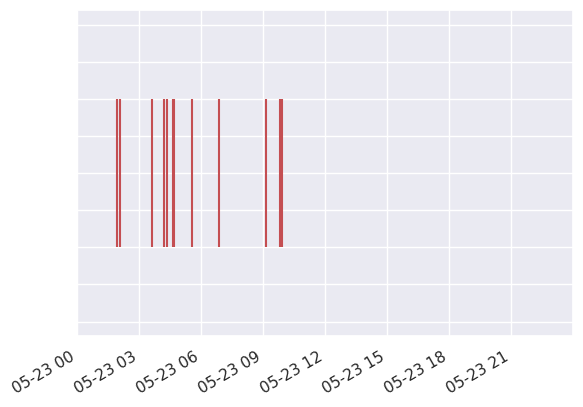
\includegraphics{Análisis_files/figure-pdf/fig-eventosddos-output-1.png}

}

\caption{\label{fig-eventosddos}Visualización de eventos de DDoS}

\end{figure}

Notar que a comparación de los por SSH parecen menos siendo que son 380
ataques contra 12. Esto es porque son muy seguido.

\hypertarget{anuxe1lisis-de-isps-1}{%
\subsubsection{Análisis de ISPs}\label{anuxe1lisis-de-isps-1}}

\begin{Shaded}
\begin{Highlighting}[]
\NormalTok{recuento }\OperatorTok{=}\NormalTok{ df[}\StringTok{"isp"}\NormalTok{].value\_counts().to\_dict()}

\NormalTok{recuento }\OperatorTok{=}\NormalTok{ pd.DataFrame(data}\OperatorTok{=}\NormalTok{\{}\StringTok{"ISP"}\NormalTok{: }\BuiltInTok{list}\NormalTok{(recuento.keys()), }\StringTok{"Reportes"}\NormalTok{: }\BuiltInTok{list}\NormalTok{(recuento.values())\})}
\NormalTok{recuento}
\end{Highlighting}
\end{Shaded}

\begin{longtable}[]{@{}lll@{}}
\toprule\noalign{}
& ISP & Reportes \\
\midrule\noalign{}
\endhead
\bottomrule\noalign{}
\endlastfoot
0 & Suniway Group Limited & 75 \\
1 & Gold Experience Cloud LLC & 75 \\
2 & Dragon Spirit Investments International Co. Li... & 73 \\
3 & WTW Hightech Company Inc & 67 \\
4 & Suniway Telecom & 39 \\
5 & Suniway Group of Companies Inc. & 36 \\
6 & Intercontinental Internet Data Corp & 1 \\
7 & Bell Canada & 1 \\
8 & Comcast Cable Communications LLC & 1 \\
9 & Cabo Servicos de Telecomunicacoes Ltda & 1 \\
10 & Shaw Communications Inc. & 1 \\
11 & Delta DCCNet High Speed Internet & 1 \\
12 & Nexus Bytes LLC & 1 \\
13 & Dot Internet & 1 \\
14 & VPSquan L.L.C. & 1 \\
15 & Kurun Cloud Inc & 1 \\
16 & Shine Telecom Co. Ltd. & 1 \\
17 & CTG Server Ltd. & 1 \\
18 & Reliablesite.net LLC & 1 \\
\end{longtable}

\begin{Shaded}
\begin{Highlighting}[]
\NormalTok{fig}\OperatorTok{=}\NormalTok{plt.plot(figsize}\OperatorTok{=}\NormalTok{(}\DecValTok{15}\NormalTok{, }\DecValTok{10}\NormalTok{))}
\NormalTok{sns.countplot(data}\OperatorTok{=}\NormalTok{df, y}\OperatorTok{=}\StringTok{"isp"}\NormalTok{)}


    
\NormalTok{plt.tick\_params(labelsize }\OperatorTok{=} \DecValTok{11}\NormalTok{)}
\CommentTok{\#plt.xticks([1,2,3])}
\NormalTok{plt.ylabel(}\StringTok{"ISPs"}\NormalTok{, rotation}\OperatorTok{=}\DecValTok{0}\NormalTok{)}
\NormalTok{plt.xlabel(}\StringTok{"Veces denunciado"}\NormalTok{)}
\NormalTok{plt.show()}
\end{Highlighting}
\end{Shaded}

\begin{figure}[H]

{\centering 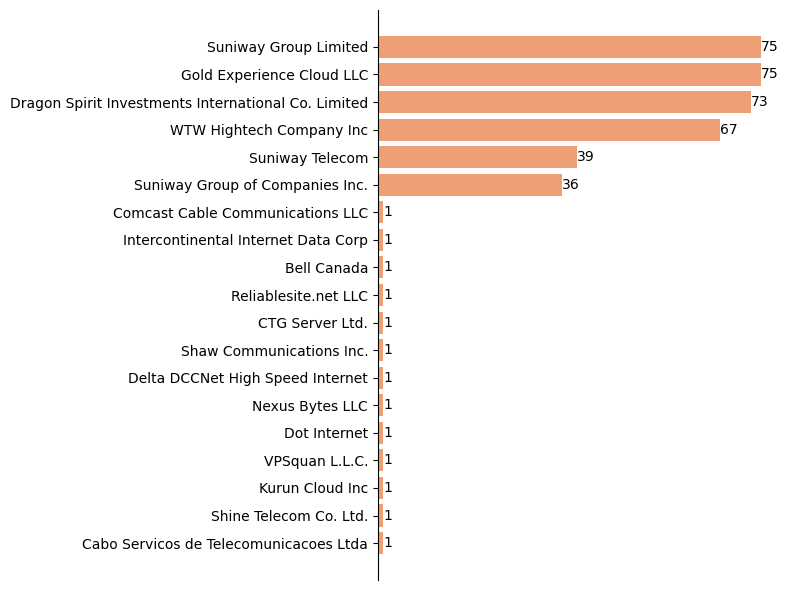
\includegraphics{Análisis_files/figure-pdf/fig-ispsddos-output-1.png}

}

\caption{\label{fig-ispsddos}Número de veces que se denuncio un ISP por
ataque DDoS}

\end{figure}

\hypertarget{anuxe1lisis-de-uso-1}{%
\subsubsection{Análisis de uso}\label{anuxe1lisis-de-uso-1}}

\begin{Shaded}
\begin{Highlighting}[]
\NormalTok{recuento }\OperatorTok{=}\NormalTok{ df[}\StringTok{"tipoDeUso"}\NormalTok{].value\_counts().to\_dict()}

\NormalTok{recuento }\OperatorTok{=}\NormalTok{ pd.DataFrame(data}\OperatorTok{=}\NormalTok{\{}\StringTok{"uso"}\NormalTok{: }\BuiltInTok{list}\NormalTok{(recuento.keys()), }\StringTok{"Reportes"}\NormalTok{: }\BuiltInTok{list}\NormalTok{(recuento.values())\})}
\NormalTok{recuento}
\end{Highlighting}
\end{Shaded}

\begin{longtable}[]{@{}lll@{}}
\toprule\noalign{}
& uso & Reportes \\
\midrule\noalign{}
\endhead
\bottomrule\noalign{}
\endlastfoot
0 & Data Center/Web Hosting/Transit & 335 \\
1 & Fixed Line ISP & 42 \\
2 & Commercial & 1 \\
\end{longtable}

\begin{Shaded}
\begin{Highlighting}[]
\NormalTok{fig, ax }\OperatorTok{=}\NormalTok{ plt.subplots()}

\CommentTok{\# Graficar las barras intercambiando los ejes}
\NormalTok{ax.barh(recuento[}\StringTok{\textquotesingle{}uso\textquotesingle{}}\NormalTok{], recuento[}\StringTok{\textquotesingle{}Reportes\textquotesingle{}}\NormalTok{], color}\OperatorTok{=}\NormalTok{[}\StringTok{\textquotesingle{}r\textquotesingle{}}\NormalTok{, }\StringTok{\textquotesingle{}g\textquotesingle{}}\NormalTok{, }\StringTok{\textquotesingle{}b\textquotesingle{}}\NormalTok{])}

\CommentTok{\# Agregar etiquetas al final de cada barra}
\ControlFlowTok{for}\NormalTok{ i, v }\KeywordTok{in} \BuiltInTok{enumerate}\NormalTok{(recuento[}\StringTok{\textquotesingle{}Reportes\textquotesingle{}}\NormalTok{]):}
\NormalTok{    ax.text(v, i, }\BuiltInTok{str}\NormalTok{(v), ha}\OperatorTok{=}\StringTok{\textquotesingle{}left\textquotesingle{}}\NormalTok{, va}\OperatorTok{=}\StringTok{\textquotesingle{}center\textquotesingle{}}\NormalTok{)}
\end{Highlighting}
\end{Shaded}

\begin{figure}[H]

{\centering 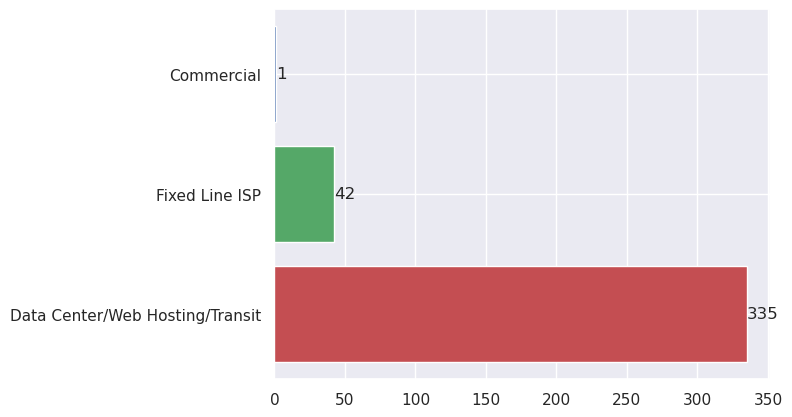
\includegraphics{Análisis_files/figure-pdf/cell-60-output-1.png}

}

\end{figure}

\hypertarget{fue-un-solo-ataque}{%
\subsubsection{¿Fue un solo ataque?}\label{fue-un-solo-ataque}}

\begin{Shaded}
\begin{Highlighting}[]
\ImportTok{import}\NormalTok{ netaddr}

\KeywordTok{def}\NormalTok{ convertirIP(ip):}
    \ControlFlowTok{return} \BuiltInTok{int}\NormalTok{(netaddr.IPAddress(ip))}
    
\end{Highlighting}
\end{Shaded}

\begin{Shaded}
\begin{Highlighting}[]
\NormalTok{datetimes }\OperatorTok{=}\NormalTok{ [evento[}\DecValTok{1}\NormalTok{] }\ControlFlowTok{for}\NormalTok{ evento }\KeywordTok{in}\NormalTok{ eventosDDoS]}
\NormalTok{dicc }\OperatorTok{=}\NormalTok{ \{}\StringTok{"ip"}\NormalTok{: df[}\StringTok{"ip"}\NormalTok{],}
        \StringTok{"datetime"}\NormalTok{: datetimes\}}
\end{Highlighting}
\end{Shaded}

\begin{Shaded}
\begin{Highlighting}[]
\NormalTok{dfClusters }\OperatorTok{=}\NormalTok{ pd.DataFrame(dicc)}
\NormalTok{dfClusters[}\StringTok{"datetime"}\NormalTok{] }\OperatorTok{=}\NormalTok{ dfClusters[}\StringTok{"datetime"}\NormalTok{].}\BuiltInTok{apply}\NormalTok{(}\KeywordTok{lambda}\NormalTok{ x: x.utcnow().timestamp())}
\NormalTok{dfClusters[}\StringTok{"ip"}\NormalTok{] }\OperatorTok{=}\NormalTok{ dfClusters[}\StringTok{"ip"}\NormalTok{].}\BuiltInTok{apply}\NormalTok{(convertirIP)}
\end{Highlighting}
\end{Shaded}

\begin{Shaded}
\begin{Highlighting}[]
\NormalTok{sns.scatterplot(data}\OperatorTok{=}\NormalTok{dfClusters,x}\OperatorTok{=}\StringTok{"datetime"}\NormalTok{, y}\OperatorTok{=}\StringTok{"ip"}\NormalTok{)}
\NormalTok{plt.xlabel(}\StringTok{"Tiempo"}\NormalTok{)}
\NormalTok{plt.ylabel(}\StringTok{"IPs"}\NormalTok{)}
\NormalTok{plt.xticks([])}
\NormalTok{plt.yticks([])}
\NormalTok{plt.show()}
\end{Highlighting}
\end{Shaded}

\begin{figure}[H]

{\centering 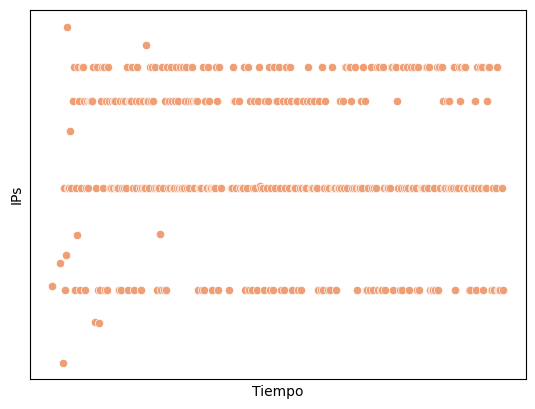
\includegraphics{Análisis_files/figure-pdf/fig-usodeips-output-1.png}

}

\caption{\label{fig-usodeips}IPs vs Tiempo}

\end{figure}

Como se puede observar en Figure~\ref{fig-usodeips} pareciese ser que a
pesar de que se realizaron reportes en horarios distantes, las IPs no
ocupan todo el espectro. Se podría inferir que fue el mismo atacante
porque uso IPs en un rango acotado



\end{document}
